\documentclass[xcolor=dvipsnames,notes]{beamer}
\usecolortheme[named=Brown]{structure}
\usetheme{default}
\setbeamertemplate{navigation symbols}{} 
\usepackage{tikz}
\usetikzlibrary{arrows,decorations.pathmorphing,backgrounds,positioning,fit}
\usetikzlibrary{datavisualization.formats.functions}
\usetikzlibrary{shapes}
%     
%Here are some macro's saving time and labour:     
%     
\newcommand{\const}{\mbox{const}}      
\newcommand{\est}{\mbox{{\tiny est}}}      
\newcommand{\im}{\mbox{$\Im \mbox{m}$}}      
\newcommand{\obs}{\mbox{{\tiny obs}}}      
\newcommand{\otherwise}{\mbox{otherwise}}      
\newcommand{\real}{\mbox{$\Re \mbox{e}$}}      
\newcommand{\sign}{\mbox{sign}}      
\newcommand{\sinc}{\mbox{sinc}}      
%
\newcommand{\p}{\mbox{$\partial$}}      
\renewcommand{\d}{\mbox{$\partial$}}      
\newcommand{\w}{\mbox{$\omega$}}      
%
\newcommand{\AAA}{\mbox{\boldmath $A$}}   
\newcommand{\BB}{\mbox{\boldmath $B$}}     
\newcommand{\CC}{\mbox{\boldmath $C$}}     
\newcommand{\DD}{\mbox{\boldmath $D$}}     
\newcommand{\EE}{\mbox{\boldmath $E$}}     
\newcommand{\FF}{\mbox{\boldmath $F$}}   
\newcommand{\GG}{\mbox{\boldmath $G$}}   
\newcommand{\HH}{\mbox{\boldmath $H$}}   
\newcommand{\II}{\mbox{\boldmath $I$}}   
\newcommand{\JJ}{\mbox{\boldmath $J$}}   
\newcommand{\KK}{\mbox{\boldmath $K$}}   
\newcommand{\LL}{\mbox{\boldmath $L$}}   
\newcommand{\MM}{\mbox{\boldmath $M$}}   
\newcommand{\NN}{\mbox{\boldmath $N$}}   
\newcommand{\OO}{\mbox{\boldmath $O$}}   
\newcommand{\PP}{\mbox{\boldmath $P$}}   
\newcommand{\QQ}{\mbox{\boldmath $Q$}}   
\newcommand{\RR}{\mbox{\boldmath $R$}}   
\newcommand{\SSS}{\mbox{\boldmath $S$}}   
\newcommand{\TT}{\mbox{\boldmath $T$}}   
\newcommand{\UU}{\mbox{\boldmath $U$}}   
\newcommand{\VV}{\mbox{\boldmath $V$}}   
\newcommand{\WW}{\mbox{\boldmath $W$}}   
\newcommand{\XX}{\mbox{\boldmath $X$}}   
\newcommand{\YY}{\mbox{\boldmath $Y$}}   
\newcommand{\ZZ}{\mbox{\boldmath $Z$}}   
%
%\newcommand{\aaa}{\mbox{\boldmath $a$}}     
\newcommand{\bb}{\mbox{\boldmath $b$}}     
\newcommand{\cc}{\mbox{\boldmath $c$}}     
\newcommand{\dd}{\mbox{\boldmath $d$}}     
\newcommand{\ee}{\mbox{\boldmath $e$}}   
\newcommand{\ff}{\mbox{\boldmath $f$}}   
%\newcommand{\ggg}{\mbox{\boldmath $g$}}   
\newcommand{\hh}{\mbox{\boldmath $h$}}   
\newcommand{\ii}{\mbox{\boldmath $i$}}   
\newcommand{\jj}{\mbox{\boldmath $j$}}   
\newcommand{\kk}{\mbox{\boldmath $k$}}   
%\newcommand{\lll}{\mbox{\boldmath $l$}}   
\newcommand{\mm}{\mbox{\boldmath $m$}}   
\newcommand{\nn}{\mbox{\boldmath $n$}}   
\newcommand{\pp}{\mbox{\boldmath $p$}}   
\newcommand{\qq}{\mbox{\boldmath $q$}}   
\newcommand{\rr}{\mbox{\boldmath $r$}}   
%\newcommand{\sss}{\mbox{\boldmath $s$}}   
%\newcommand{\ttt}{\mbox{\boldmath $t$}}   
\newcommand{\uu}{\mbox{\boldmath $u$}}   
\newcommand{\vv}{\mbox{\boldmath $v$}}   
\newcommand{\ww}{\mbox{\boldmath $w$}}   
\newcommand{\xx}{\mbox{\boldmath $x$}}   
\newcommand{\yy}{\mbox{\boldmath $y$}}   
\newcommand{\zz}{\mbox{\boldmath $z$}}   
%
\newcommand{\balpha}{\mbox{\boldmath $\alpha$}}     
\newcommand{\bpsi}{\mbox{\boldmath $\psi$}}     
\newcommand{\bphi}{\mbox{\boldmath $\phi$}}     
\newcommand{\bbeta}{\mbox{\boldmath $\beta$}}     
\newcommand{\btheta}{\mbox{\boldmath $\theta$}}     
\newcommand{\bdelta}{\mbox{\boldmath $\delta$}}     
\newcommand{\bgamma}{\mbox{\boldmath $d$}}     
\newcommand{\bGamma}{\mbox{\boldmath $\Gamma$}}     
\newcommand{\bLambda}{\mbox{\boldmath $\Lambda$}}     
\newcommand{\bmu}{\mbox{\boldmath $\mu$}}     
\newcommand{\bnabla}{\mbox{\boldmath $\nabla$}}     
\newcommand{\brho}{\mbox{\boldmath $\rho$}}     
\newcommand{\bSigma}{\mbox{\boldmath $\Sigma$}}     
\newcommand{\bsigma}{\mbox{\boldmath $\sigma$}}     
\newcommand{\bxi}{\mbox{\boldmath $\xi$}}     
\newcommand{\bepsilon}{\mbox{\boldmath $\epsilon$}}     
\newcommand{\blambda}{\mbox{\boldmath $\lambda$}}     
\newcommand{\BLambda}{\mbox{\boldmath $\Lambda$}}     
%-------------------------------------%
%  \Appendix - a new appendix command %
%-------------------------------------%
%The appendix command is used as in
% \Appendix{A}{The wave equation as a matrix equation}
\newcommand {\Appendix}[1]{
              \section*{APPENDIX #1}
              \setcounter{equation}{0}
              \renewcommand{\theequation} 
              {A-\arabic{equation}}}
\newcommand {\Appendices}[2]{
              \section*{APPENDIX #1: #2 }
              \setcounter{equation}{0}
              \renewcommand{\theequation} 
              {#1-\arabic{equation}}}
%------------------------------------%
%    \aref - a new cite command.     % 
%------------------------------------%
\newcommand{\aref}[2]{\nocite{#1}#2} 
%----------------------------------------
%\eqref -an equation reference command
%----------------------------------------
%\newcommand{\eqref}[1]{(\ref{#1})}
%\newcommand{\eqref}[1]{\ref{#1}}

\usepackage{epsfig}
\usepackage{natbib}
\usepackage{graphicx}
\usepackage{multimedia}
\usepackage{verbatim}
\include{acmmacro}
\begin{document}
%\setbeamercolor{titlelike}{fg=gray,bg=white}
%\setbeamercolor{itemize item}{fg=gray,bg=white}
%\setbeamercolor{enumerate item}{fg=gray,bg=white}
%\setbeamercolor{block title}{fg=black,bg=white}
%==============================================
\title{TPG4190 Seismic data acquisition and processing \\
               Imaging}
\author{B. Arntsen}
\institute[NTNU]{
  NTNU\\
  Department of Geoscience and petroleum \\
  \texttt{borge.arntsen@ntnu.no}
}
\date{Trondheim fall 2023}
\begin{frame}
 \titlepage
\end{frame}
%
%==============================================
\begin{frame}{Overview}
%==============================================
\begin{itemize}
  \item Imaging conditions 
  \item Reciprocity 
  \item Time reversal 
  \item Imaging formula 
  \end{itemize}
\end{frame}
%-----------------------------------------
\begin{frame}{Imaging condition I}
%-----------------------------------------
\begin{figure}
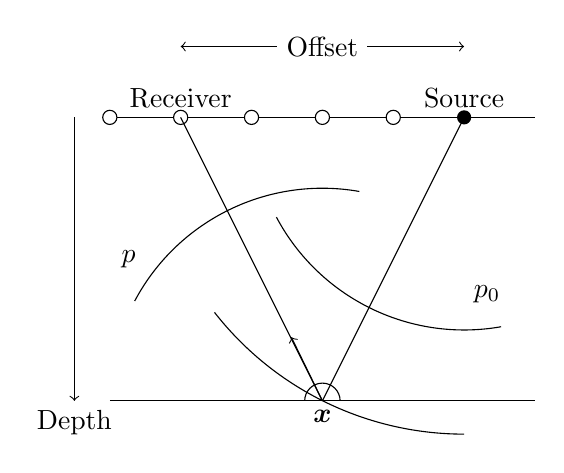
\begin{tikzpicture}[scale=0.9]
  \draw[->] (-0.5,4.0) -- (-0.5,0.0) node[below]{Depth} ;
  \draw[<->] (1.0,5.0) -- node[fill=white]{Offset} (5.0,5.0); 
  \draw (0.0,0.0) -- (6.0,0.0) ;
  \draw (0.0,4.0) -- (6.0,4.0) ;
  \fill (5.0,4.0) node[above]{Source} circle (0.1) ;
  \fill[white] (0.0,4.0) circle (0.1) ;
  \draw (0.0,4.0) circle (0.1) ;
  \fill[white](1.0,4.0) circle (0.1) ;
  \draw (1.0,4.0) node[above]{Receiver}circle (0.1) ;
  \fill[white] (2.0,4.0) circle (0.1) ;
  \draw (2.0,4.0) circle (0.1) ;
  \fill[white] (3.0,4.0) circle (0.1) ;
  \draw (3.0,4.0) circle (0.1) ;
  \fill[white] (4.0,4.0) circle (0.1) ;
  \draw (4.0,4.0) circle (0.1) ;
  \draw (5.0,4.0) -- (3.0,0.0) ;
  \draw (3.0,0.0) -- (1.0,4.0) ;
% Upgoing wave circle
  \draw (3,0) +(80:3) arc(80:152:3);
  \draw (3,0) +(0:0.25) arc(0:180:0.25);
  \draw (5,4) +(-80:3) arc(-80:-152:3);
  \draw (5,4) +(-90:4.47) arc(-90:-142:4.47);
  \draw (5.0,1.5) node[right]{$p_0$};
  \draw (0.5,2.0) node[left]{$p$};
  \draw (3,0) node[below]{$\xx$};
  %\draw (3.4,0.125) node[below]{$\xx'$};
  \draw[->] (3,0)-- +(116:1);
\end{tikzpicture}
%\label{fig:si-1}
\end{figure}
$p$: Scattereded wavefield (data)\\
$p_0$: Modeled wavefield\\
$\xx$: Spatial position
\end{frame}
%-----------------------------------------
\begin{frame}{Imaging condition II}
%-----------------------------------------
\begin{figure}
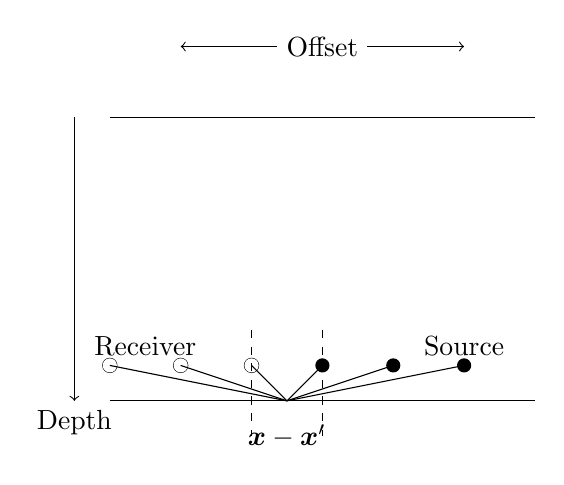
\begin{tikzpicture}[scale=0.9]
   \draw[->] (-0.5,4.0) -- (-0.5,0.0) node[below]{Depth} ;      %Depth axis 
   \draw[<->] (1.0,5.0) -- node[fill=white]{Offset} (5.0,5.0);  %Offset axis  
  \draw (0.0,4.0) -- (6.0,4.0) ;                               % Boundary at top
  \draw (0.0,0.0) -- (6.0,0.0) ;                               % Boundary at depth

  \fill (3.0,0.5) node[above]{} circle (0.1) ;           % Draw source
  \fill (4.0,0.5) node[above]{} circle (0.1) ;           % Draw source
  \fill (5.0,0.5) node[above]{Source} circle (0.1) ;     % Draw source text

  \draw (2.0,0.5) circle (0.1) ;             %Draw receiver
  \fill[white] (2.0,0.5) circle (0.1) ;

  \draw (1.0,0.5) circle (0.1) ;             %Draw receiver
  \fill[white] (1.0,0.5) circle (0.1) ;

  \draw (0.0,0.5) circle (0.1) ;             %Draw receiver
  \fill[white] (0.0,0.5) circle (0.1) ;
  \draw (0.5,0.5) node[above]{Receiver} ;    %Draw receiver text 

  \draw (3.0,0.5) -- (2.5,0.0);              % Draw ray from source to midpoint
  \draw (4.0,0.5) -- (2.5,0.0);              % Draw ray from source to midpoint
  \draw (5.0,0.5) -- (2.5,0.0);              % Draw ray from source to midpoint

  \draw (2.0,0.5) -- (2.5,0.0);              % Draw ray from receiver to midpoint
  \draw (1.0,0.5) -- (2.5,0.0);              % Draw ray from receiver to midpoint
  \draw (0.0,0.5) -- (2.5,0.0);              % Draw ray from receiver to midpoint

  \draw[dashed] (2.0,1.0) -- (2.0,-0.5);     %Draw vertical dashed line
  \draw[dashed] (3.0,1.0) -- (3.0,-0.5);     %Draw vertical dashed line
  \draw (2.5,-0.5) node {$\xx-\xx'$};           % Draw equation

\end{tikzpicture}
%\label{fig:si-1}

$\xx$: Virtual receiver\\
$\xx'$: Virtual source
\end{figure}
\end{frame}
%-----------------------------------------
\begin{frame}{Imaging condition III}
%-----------------------------------------
\begin{figure}
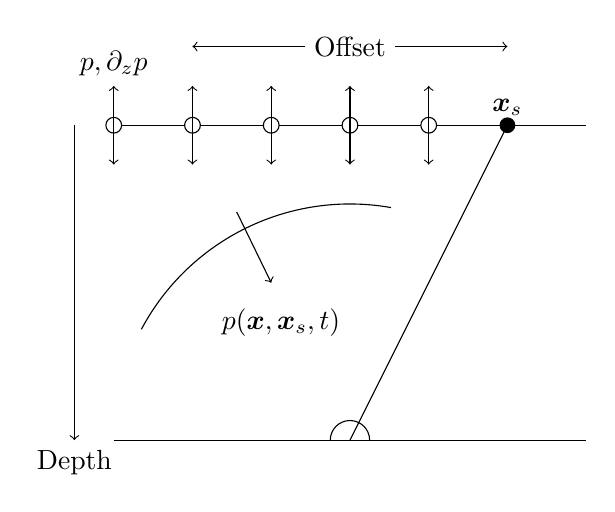
\begin{tikzpicture}[scale=1.0]
  \draw[->] (-0.5,4.0) -- (-0.5,0.0) node[below]{Depth} ;     %Draw Depth axis
  \draw[<->] (1.0,5.0) -- node[fill=white]{Offset} (5.0,5.0); %Draw offset axis 
  \draw (0.0,0.0) -- (6.0,0.0) ;  %Top boundary
  \draw (0.0,4.0) -- (6.0,4.0) ;  %Bottom boundary

  \fill (5.0,4.0) node[above]{$\xx_s$} circle (0.1) ; % Draw source

  \fill[white] (0.0,4.0) circle (0.1) ; %Draw receiver
  \draw (0.0,4.0) circle (0.1) ;
  \draw[->] (0.0,4.0) -- (0.0,4.5);
  \draw[->] (0.0,4.0) -- (0.0,3.5);
  \draw (0.0,4.5) node[above]{$p,\partial_z p$};
  

  \fill[white](1.0,4.0) circle (0.1) ;
  \draw (1.0,4.0) node[above]{} circle (0.1) ;
  \draw[->] (1.0,4.0) -- (1.0,4.5);
  \draw[->] (1.0,4.0) -- (1.0,3.5);

  \fill[white] (2.0,4.0) circle (0.1) ;
  \draw (2.0,4.0) circle (0.1) ;
  \draw[->] (2.0,4.0) -- (2.0,4.5);
  \draw[->] (2.0,4.0) -- (2.0,3.5);

  \fill[white] (3.0,4.0) circle (0.1) ;
  \draw (3.0,4.0) circle (0.1) ;
  \draw[->] (3.0,4.0) -- (3.0,4.5);
  \draw[->] (3.0,4.0) -- (3.0,3.5);

  \fill[white] (4.0,4.0) circle (0.1) ;
  \draw (4.0,4.0) circle (0.1) ;
  \draw[->] (4.0,4.0) -- (4.0,4.5);
  \draw[->] (4.0,4.0) -- (4.0,3.5);

  \draw[<-] (2,2)-- +(116:1);
  \draw (3,0) +(0:0.25) arc(0:180:0.25);
  \draw (3,0) +(80:3) arc(80:152:3);
  \draw (3.0,1.5) node[left]{$p(\xx,\xx_s,t)$};


  \draw (5.0,4.0) -- (3.0,0.0) ;
  %\draw (3.0,0.0) -- (1.0,4.0) ;
\end{tikzpicture}
%\label{fig:si-1}

$p$: Scattered wavefield \\
$\xx_s$: Source position\\
$\xx,t$: Position,time
\end{figure}
\end{frame}
%-----------------------------------------
\begin{frame}{Imaging condition IV}
%-----------------------------------------
\begin{figure}
\begin{tikzpicture}[scale=1.0]
  \draw[->] (-0.5,4.0) -- (-0.5,0.0) node[below]{Depth} ;     %Draw Depth axis
  \draw[<->] (1.0,5.0) -- node[fill=white]{Offset} (5.0,5.0); %Draw offset axis 
  \draw (0.0,0.0) -- (6.0,0.0) ;  %Top boundary
  \draw (0.0,4.0) -- (6.0,4.0) ;  %Bottom boundary

  \fill (5.0,4.0) node[above]{$\xx_s$} circle (0.1) ; % Draw source

  \fill[white] (0.0,0.5) circle (0.1) ; %Draw receiver
  \draw (0.0,0.5) circle (0.1) ;
  

  \fill[white](1.0,0.5) circle (0.1) ;
  \draw (1.0,0.5) node[above]{} circle (0.1) ;

  \fill[white] (2.0,0.5) circle (0.1) ;
  \draw (2.0,0.5) circle (0.1) ;

%  \fill[white] (3.0,0.5) circle (0.1) ;
%  \draw (3.0,0.5) circle (0.1) ;

%  \fill[white] (4.0,0.5) circle (0.1) ;
%  \draw (4.0,0.5) circle (0.1) ;

  \draw[->] (3,0)-- (0.0,0.5);
  \draw[->] (3,0)-- (1.0,0.5);
  \draw[->] (3,0)-- (2.0,0.5);
  %\draw[->] (3,0)-- (3.0,0.5);
  %\draw[->] (3,0)-- (4.0,0.5);
%  \draw (3,0) +(0:0.25) arc(0:180:0.25);
%  \draw (3,0) +(80:3) arc(80:152:3);
  \draw (3.0,1.5) node[left]{$(\xx,\xx_s,t)$};


  \draw (5.0,4.0) -- (3.0,0.0) ;
  %\draw (3.0,0.0) -- (1.0,4.0) ;
\end{tikzpicture}
%\label{fig:si-1}
\end{figure}
\end{frame}
%-----------------------------------------
\begin{frame}{Imaging condition V}
%-----------------------------------------
\begin{figure}
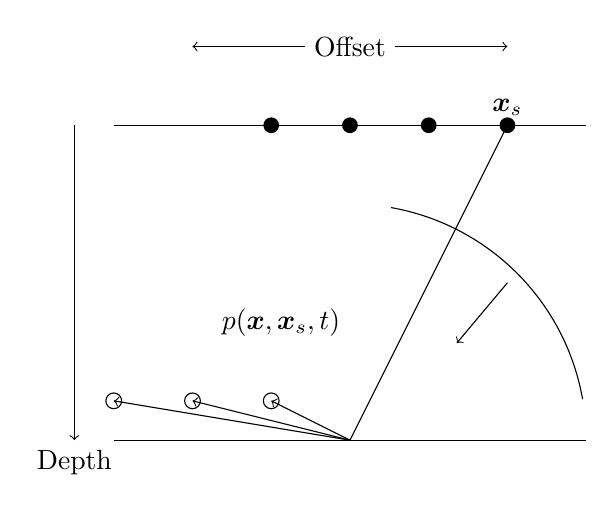
\begin{tikzpicture}[scale=1.0]
  \draw[->] (-0.5,4.0) -- (-0.5,0.0) node[below]{Depth} ;     %Draw Depth axis
  \draw[<->] (1.0,5.0) -- node[fill=white]{Offset} (5.0,5.0); %Draw offset axis 
  \draw (0.0,0.0) -- (6.0,0.0) ;  %Top boundary
  \draw (0.0,4.0) -- (6.0,4.0) ;  %Bottom boundary

  \fill (5.0,4.0) node[above]{$\xx_s$} circle (0.1) ; % Draw source
  \fill (4.0,4.0) node[above]{} circle (0.1) ; % Draw source
  \fill (3.0,4.0) node[above]{} circle (0.1) ; % Draw source
  \fill (2.0,4.0) node[above]{} circle (0.1) ; % Draw source

  \fill[white] (0.0,0.5) circle (0.1) ; %Draw receiver
  \draw (0.0,0.5) circle (0.1) ;
  

  \fill[white](1.0,0.5) circle (0.1) ;
  \draw (1.0,0.5) node[above]{} circle (0.1) ;

  \fill[white] (2.0,0.5) circle (0.1) ;
  \draw (2.0,0.5) circle (0.1) ;

%  \fill[white] (3.0,0.5) circle (0.1) ;
%  \draw (3.0,0.5) circle (0.1) ;

%  \fill[white] (4.0,0.5) circle (0.1) ;
%  \draw (4.0,0.5) circle (0.1) ;

  \draw[->] (3,0)-- (0.0,0.5);
  \draw[->] (3,0)-- (1.0,0.5);
  \draw[->] (3,0)-- (2.0,0.5);
%  \draw[->] (3,0)-- (3.0,0.5);
%  \draw[->] (3,0)-- (4.0,0.5);
%  \draw (3,0) +(0:0.25) arc(0:180:0.25);
%  \draw (3,0) +(80:3) arc(80:152:3);
  \draw (3.0,1.5) node[left]{$p(\xx,\xx_s,t)$};
\draw (3,0) +(80:3) arc(80:10:3);

  \draw[->] (5,2)-- +(230:1);

  \draw (5.0,4.0) -- (3.0,0.0) ;
  %\draw (3.0,0.0) -- (1.0,4.0) ;
\end{tikzpicture}
%\label{fig:si-1}
\end{figure}
\end{frame}
%-----------------------------------------
\begin{frame}{Imaging condition VI}
%-----------------------------------------
\begin{figure}
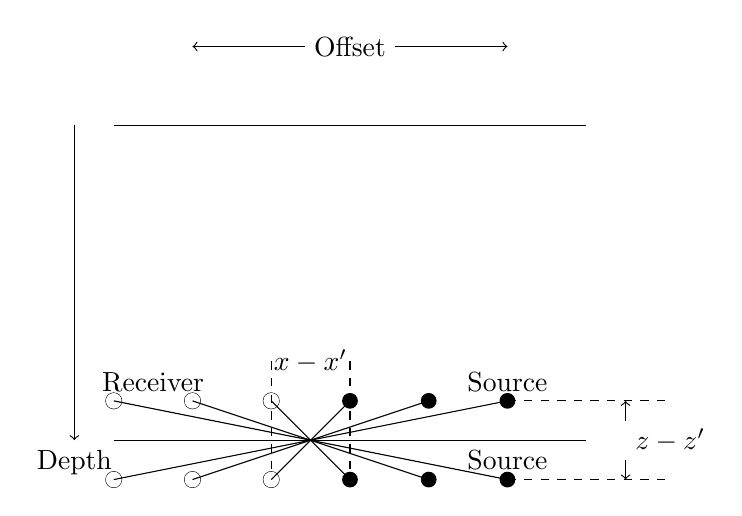
\begin{tikzpicture}[scale=1.0]
   \draw[->] (-0.5,4.0) -- (-0.5,0.0) node[below]{Depth} ;      %Depth axis 
   \draw[<->] (1.0,5.0) -- node[fill=white]{Offset} (5.0,5.0);  %Offset axis  
  \draw (0.0,4.0) -- (6.0,4.0) ;                               % Boundary at top
  \draw (0.0,0.0) -- (6.0,0.0) ;                               % Boundary at depth

  \fill (3.0,0.5) node[above]{} circle (0.1) ;           % Draw source
  \fill (4.0,0.5) node[above]{} circle (0.1) ;           % Draw source
  \fill (5.0,0.5) node[above]{Source} circle (0.1) ;     % Draw source text

  \draw (2.0,0.5) circle (0.1) ;             %Draw receiver
  \fill[white] (2.0,0.5) circle (0.1) ;

  \draw (1.0,0.5) circle (0.1) ;             %Draw receiver
  \fill[white] (1.0,0.5) circle (0.1) ;

  \draw (0.0,0.5) circle (0.1) ;             %Draw receiver
  \fill[white] (0.0,0.5) circle (0.1) ;
  \draw (0.5,0.5) node[above]{Receiver} ;    %Draw receiver text 

  \draw (3.0,0.5) -- (2.5,0.0);              % Draw ray from source to midpoint
  \draw (4.0,0.5) -- (2.5,0.0);              % Draw ray from source to midpoint
  \draw (5.0,0.5) -- (2.5,0.0);              % Draw ray from source to midpoint

  \draw (2.0,0.5) -- (2.5,0.0);              % Draw ray from receiver to midpoint
  \draw (1.0,0.5) -- (2.5,0.0);              % Draw ray from receiver to midpoint
  \draw (0.0,0.5) -- (2.5,0.0);              % Draw ray from receiver to midpoint

  \draw[dashed] (2.0,1.0) -- (2.0,-0.5);     %Draw vertical dashed line
  \draw[dashed] (3.0,1.0) -- (3.0,-0.5);     %Draw vertical dashed line
  \draw (2.5,1.0) node {$x-x'$};           % Draw equation
  \draw[dashed] (5.0,0.5) -- (7.0,0.5);     %Draw vertical dashed line
  \draw[dashed] (5.0,-0.5) -- (7.0,-0.5);     %Draw vertical dashed line
  \draw (6.5,0.0) node[right]{$z-z'$};           % Draw equation
  \draw[->] (6.5,0.25) -- (6.5,0.5);
  \draw[->] (6.5,-0.25) -- (6.5,-0.5);



  \fill (3.0,-0.5) node[above]{} circle (0.1) ;           % Draw source
  \fill (4.0,-0.5) node[above]{} circle (0.1) ;           % Draw source
  \fill (5.0,-0.5) node[above]{Source} circle (0.1) ;     % Draw source text

  \draw (2.0,-0.5) circle (0.1) ;             %Draw receiver
  \fill[white] (2.0,-0.5) circle (0.1) ;

  \draw (1.0,-0.5) circle (0.1) ;             %Draw receiver
  \fill[white] (1.0,-0.5) circle (0.1) ;

  \draw (0.0,-0.5) circle (0.1) ;             %Draw receiver
  \fill[white] (0.0,-0.5) circle (0.1) ;
  %\draw (0.5,0.5) node[above]{Receiver} ;    %Draw receiver text 

  \draw (3.0,-0.5) -- (2.5,0.0);              % Draw ray from source to midpoint
  \draw (4.0,-0.5) -- (2.5,0.0);              % Draw ray from source to midpoint
  \draw (5.0,-0.5) -- (2.5,0.0);              % Draw ray from source to midpoint

  \draw (2.0,-0.5) -- (2.5,0.0);              % Draw ray from receiver to midpoint
  \draw (1.0,-0.5) -- (2.5,0.0);              % Draw ray from receiver to midpoint
  \draw (0.0,-0.5) -- (2.5,0.0);              % Draw ray from receiver to midpoint
\end{tikzpicture}
\end{figure}

$x-x'$: Horizontal offset \\
$z-z'$: Vertical offset 
\end{frame}
%-----------------------------------------
\begin{frame}{Reciprocity}
%-----------------------------------------
\begin{figure}
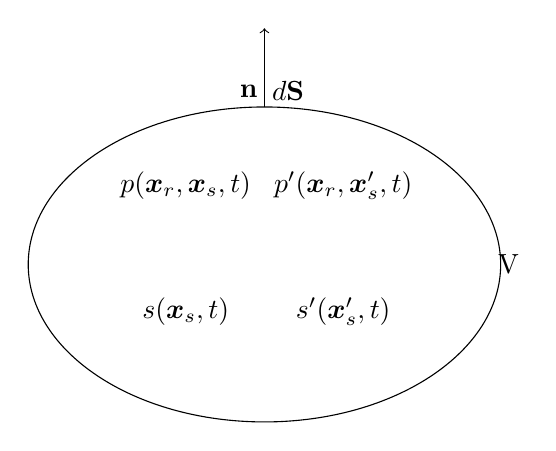
\begin{tikzpicture}
\draw (0,0) ellipse (3cm and 2cm);
\draw (3.1,0) node{V};
\draw (0.3,2.2) node {$d\mathbf{S}$};
\draw (-0.2,2.2) node {$\mathbf{n}$};
\draw[->] (0.0,2.0) -- (0.0,3.0);
\draw (-1.0,1.0) node {$p(\xx_r,\xx_s,t)$};
\draw (1.0,1.0) node {$p'(\xx_r,\xx'_s,t)$};
\draw (1.0,-0.6) node {$s'(\xx_s',t)$};
\draw (-1.0,-0.6) node {$s(\xx_s,t)$};
\end{tikzpicture}
\end{figure}
\end{frame}
%-----------------------------------------
\begin{frame}{Reciprocity}
%-----------------------------------------
\begin{figure}
\begin{tikzpicture}[scale=1.0]
  %Draw boundary S
  \draw (-0.5,4.0) -- (-0.5,-2.0) node[below]{Depth} ;   %Draw left depth axis
  \draw (6.5,4.0) -- (6.5,-2.0)   ;   %Draw right Depth axis
  \draw (-0.5,4.0) -- (6.5,4.0)   ;   %Draw upper horizontal axis
  \draw (-0.5,-2.0) -- (6.5,-2.0) ;   %Draw lower horisontal axis
  \draw (0.0,0.0) -- (6.0,0.0)    ;  % Draw Reflector
  \draw[<->] (1.0,5.0) -- node[fill=white]{Offset} (5.0,5.0); %Draw offset axis 

  \fill (5.0,3.5) node[above]{$\xx_s$} circle (0.1) ; % Draw source
  \draw (5.0,3.5) -- (3.0,0.0) ; %Draw ray from source to point R

  %Draw receiver 1
  \fill[white] (0.0,4.0) circle (0.1) ; 
  \draw (0.0,4.0) circle (0.1) ;
  \draw[->] (0.0,4.0) -- (0.0,4.5);
  \draw[->] (0.0,4.0) -- (0.0,3.5);
  \draw (0.0,4.5) node[above]{$p,\partial_z p$};

  %Draw receiver 2
  \fill[white](1.0,4.0) circle (0.1) ;
  \draw (1.0,4.0) node[above]{} circle (0.1) ;
  \draw[->] (1.0,4.0) -- (1.0,4.5);
  \draw[->] (1.0,4.0) -- (1.0,3.5);

  %Draw receiver 3
  \fill[white] (2.0,4.0) circle (0.1) ;
  \draw (2.0,4.0) circle (0.1) ;
  \draw[->] (2.0,4.0) -- (2.0,4.5);
  \draw[->] (2.0,4.0) -- (2.0,3.5);

  %Draw receiver 4
  \fill[white] (3.0,4.0) circle (0.1) ;
  \draw (3.0,4.0) circle (0.1) ;
  \draw[->] (3.0,4.0) -- (3.0,4.5);
  \draw[->] (3.0,4.0) -- (3.0,3.5);

  %Draw (small) reflected wave at point R
  \fill[white] (4.0,4.0) circle (0.1) ;
  \draw (4.0,4.0) circle (0.1) ;
  \draw[->] (4.0,4.0) -- (4.0,4.5);
  \draw[->] (4.0,4.0) -- (4.0,3.5);

  %Draw backpropagated wave 
  \draw[<-] (2,2)-- +(116:1);
  \draw (3,0) +(0:0.25) arc(0:180:0.25);
  \draw (3,0) +(80:3) arc(80:152:3);

  %Draw Volume V annotation
  \draw (4.0,1.0) node {$V$};
  \draw (7.0,0.0) node[right] {$S$};
  \draw (6.5,0.0) -- (7.0,0.0);
\end{tikzpicture}
\end{figure}
\end{frame}
%-----------------------------------------
\begin{frame}{Reciprocity}
%-----------------------------------------
Two sources $s'$ and $s$ are located inside a volume $V$ with surface $S$
at positions $\xx_s$ and $\xx'_s$.
The corresponding wavefields are $p(\xx,\xx_s)$ and $p'(\xx,\xx'_s)$.
The wave equations for these two fields are
\begin{eqnarray}
\nabla^2 p(\xx,\xx_s,t) - \frac{1}{c^2(\xx)} \partial^2_t p(\xx,\xx_s,t) = s(\xx,t) \label{eq:we1} ,\\ 
\nabla^2 p'(\xx,\xx'_s,t) - \frac{1}{{c'}^2(\xx)} \partial^2_t p'(\xx,\xx'_s,t) = s'(\xx,t) \label{eq:we2} 
\end{eqnarray}
\end{frame}
%-----------------------------------------
\begin{frame}{Reciprocity}
%-----------------------------------------
Fourier transform over time ($\partial^2_t \rightarrow -\omega^2$)
\begin{eqnarray}
\nabla^2 P(\xx,\xx_s,\omega) + \frac{\omega^2}{c^2(\xx)} P(\xx,\xx_s,\omega) = S(\xx,\omega)\label{eq:1}  ,\\ 
\nabla^2 P'(\xx,\xx'_s,\omega) + \frac{\omega^2}{{c'}^2(\xx)} P'(\xx,\xx'_s,\omega) = S'(\xx,\omega) \label{eq:2}
\end{eqnarray}
\end{frame}
%-----------------------------------------
\begin{frame}{Reciprocity}
%-----------------------------------------
Multiply equation \eqref{eq:1} with $P'$ and equation \eqref{eq:2} with $P$ and integrate over $V$ (suppressing $\omega$ as an argument)
\begin{eqnarray}
\int dV(\xx)\, \left[P'(\xx,\xx'_s)\nabla^2 P(\xx,\xx_s) + P'(\xx,\xx'_s)\frac{\omega^2}{c^2(\xx)} P(\xx,\xx_s)\right]  & = & \nonumber \\ 
                                                                                                              \int dV(\xx)\, P'(\xx,\xx'_s)S(\xx)\label{eq:3}&&  \\ 
\int dV(\xx)\, \left[P(\xx,\xx_s)\nabla^2 P'(\xx,\xx'_s) + P(\xx,\xx_s)\frac{\omega^2}{{c'}^2(\xx)} P'(\xx,\xx'_s)\right]  & = &\nonumber\\ 
                                                                                                               \int dV(\xx) P(\xx,\xx_s)S'(\xx)&& \label{eq:4} 
\end{eqnarray}
\end{frame}
%-----------------------------------------
\begin{frame}{Reciprocity}
%-----------------------------------------
Subtract equation \eqref{eq:4} from equation \eqref{eq:3}:
(Assume $c'=c$).
\begin{eqnarray}
\int dV(\xx)\, \left[P'(\xx,\xx'_s)\nabla^2 P(\xx,\xx_s)-P(\xx,\xx_s)\nabla^2 P'(\xx,\xx'_s)\right] = \nonumber\\
       \int dV(\xx)\, \left[P'(\xx,\xx'_s)S(\xx) -P(\xx,\xx_s)S'(\xx)\right]
                   \label{eq:100}
\end{eqnarray}
\end{frame}
%-----------------------------------------
\begin{frame}{Reciprocity}
%-----------------------------------------
Gauss divergence theorem:
\begin{eqnarray}
 \int dV(\xx) \nabla \cdot \AAA(\xx) =
 \int dS\, \AAA(\xx) \cdot \nn(\xx) 
\end{eqnarray}
Put $\AAA = P'(\xx,\xx'_s) \cdot \nabla P(\xx,\xx_s)$ to get
\begin{eqnarray}
 \int dV(\xx) \nabla\left[P'(\xx,\xx'_s)\nabla P(\xx,\xx_s)\right]= &&\nonumber\\   
 \int dV(\xx) \left[P'(\xx,\xx'_s)\nabla^2 P(\xx,\xx'_s) + \nabla P'(\xx,\xx'_s)\cdot\nabla P(\xx,\xx_s)\right] = &&\nonumber\\
 \int dS\, P'(\xx,\xx'_s)\nabla P(\xx,\xx_s)\cdot \nn(\xx)&& 
                     \label{eq:10}
\end{eqnarray}
\end{frame}
%-----------------------------------------
\begin{frame}{Reciprocity}
%-----------------------------------------
Put $\AAA = P(\xx,\xx_s) \cdot \nabla P'(\xx,\xx'_s)$ to get
\begin{eqnarray}
 \int dV(\xx) \nabla\left[P(\xx,\xx_s)\nabla P'(\xx,\xx'_s)\right]= &&\nonumber\\   
 \int dV(\xx) \left[P(\xx,\xx_s)\nabla^2 P'(\xx,\xx'_s) + \nabla P'(\xx,\xx'_s)\cdot\nabla P(\xx,\xx_s)\right] = &&\nonumber\\
 \int dS\, P(\xx,\xx_s)\nabla P'(\xx,\xx'_s)\cdot \nn(\xx)&& 
                     \label{eq:20}
\end{eqnarray}
Subtract equation \eqref{eq:20} fro equation \eqref{eq:10} to get
\begin{eqnarray}
 \int dV(\xx) \left[P'(\xx,\xx'_s)\nabla^2 P(\xx,\xx_s) -  P(\xx,\xx_s)\nabla^2 P'(\xx,\xx'_s)\right]= \nonumber\\
 \int dS\, \left[P'(\xx,\xx'_s)\nabla P(\xx,\xx_s) - P(\xx,\xx_s)\nabla P'(\xx,\xx'_s)\right]\cdot \nn(\xx)
       \label{eq:200}
\end{eqnarray}
\end{frame}
%-----------------------------------------
\begin{frame}{Reciprocity}
%-----------------------------------------
Replace the left hand side of equation \eqref{eq:100} with equation \eqref{eq:200}to get
\begin{eqnarray}
\int dS(\xx)\, \left[P'(\xx,\xx'_s)\nabla P(\xx,\xx_s)-P(\xx,\xx_s)\nabla P'(\xx,\xx'_s)\right]\cdot \nn(\xx) = \nonumber\\
       \int dV(\xx)\, \left[P'(\xx,\xx'_s)S(\xx) -P(\xx,\xx_s)S'(\xx)\right]
                   \label{eq:300}
\end{eqnarray}
Assume point source $S'(\xx) = \delta(\xx-\xx'_s)$
to get
\begin{eqnarray}
   P(\xx'_s,\xx_s) = \int dV(\xx) P'(\xx,\xx'_s)S(\xx) \nonumber\\
               +\int dS(\xx)\, \left[P'(\xx,\xx'_s)\nabla P(\xx,\xx_s)-
              P(\xx,\xx_s)\nabla P'(\xx,\xx'_s)\right]\cdot \nn(\xx) \label{eq:320}
\end{eqnarray}
\end{frame}
%-----------------------------------------
\begin{frame}{Reciprocity}
%-----------------------------------------
\begin{figure}
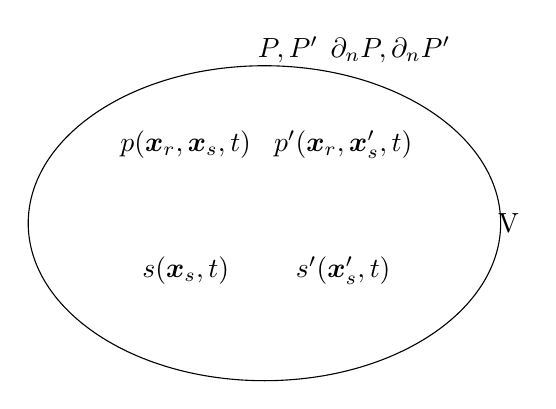
\begin{tikzpicture}
\draw (0,0) ellipse (3cm and 2cm);
\draw (3.1,0) node{V};
\draw (0.3,2.2) node {$P,P'$};
\draw (1.6,2.2) node {$\partial_n P,\partial_n P'$};
\draw (-1.0,1.0) node {$p(\xx_r,\xx_s,t)$};
\draw (1.0,1.0) node {$p'(\xx_r,\xx'_s,t)$};
\draw (1.0,-0.6) node {$s'(\xx_s',t)$};
\draw (-1.0,-0.6) node {$s(\xx_s,t)$};
\end{tikzpicture}
\end{figure}
\end{frame}
%-----------------------------------------
\begin{frame}{Reciprocity}
%-----------------------------------------
\begin{figure}
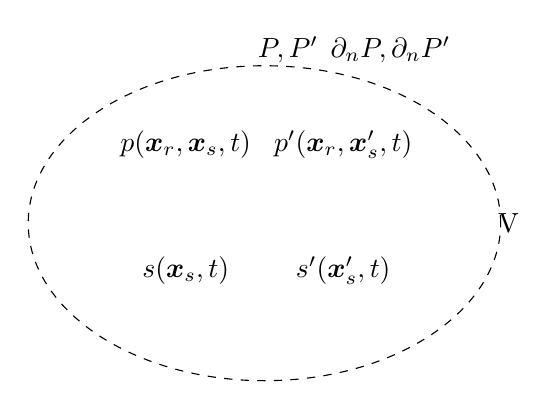
\begin{tikzpicture}
\draw[dashed] (0,0) ellipse (3cm and 2cm);
\draw (3.1,0) node{V};
\draw (0.3,2.2) node {$P,P'$};
\draw (1.6,2.2) node {$\partial_n P,\partial_n P'$};
\draw (-1.0,1.0) node {$p(\xx_r,\xx_s,t)$};
\draw (1.0,1.0) node {$p'(\xx_r,\xx'_s,t)$};
\draw (1.0,-0.6) node {$s'(\xx_s',t)$};
\draw (-1.0,-0.6) node {$s(\xx_s,t)$};
\end{tikzpicture}
\end{figure}
\end{frame}
%-----------------------------------------
\begin{frame}{Source-receiver reciprocity}
%-----------------------------------------
Assume noe that the surface integral is zero 
and that $S(\xx) = \delta(\xx-\xx_s)$. Equation \eqref{eq:300} then gives
if we assume $P=P'$ and $S=S'$
\begin{eqnarray}
   P(\xx_s,\xx'_s) =P(\xx'_s,\xx_s) 
\end{eqnarray}
The pressure recorded at $\xx_s$ due to a source at $\xx'_s$ is
the same as the pressure recorded at $\xx'_s$ due to a source at $\xx_s$.
\end{frame}
%-----------------------------------------
\begin{frame}{Reciprocity}
%-----------------------------------------
We now assume that the source of $P'$ is
\begin{eqnarray}
 S'(\xx) = \delta(\xx-\xx_s)\delta(t)
\end{eqnarray}

$P'(\xx,\xx'_s) = G(\xx,\xx'_s)$ is then 
called a Green's function.
\end{frame}
%-----------------------------------------
\begin{frame}{Reciprocity}
%-----------------------------------------
Use reciprocity $G(\xx'_s,\xx)=G(\xx,\xx'_s)$
to get from equation \eqref{eq:320}
\begin{eqnarray}
   P(\xx'_s,\xx_s) = \int dV(\xx) G(\xx'_s,\xx)S(\xx) \nonumber\\
               +\int dS(\xx)\, \left[G(\xx'_s,\xx)\nabla P(\xx,\xx_s)-
              P(\xx,\xx_s)\nabla G(\xx'_s,\xx)\right]\cdot \nn(\xx) \nonumber
\end{eqnarray}
Rename $\xx \rightarrow \xx'$ and $\xx'_s \rightarrow \xx$.
\begin{eqnarray}
   P(\xx,\xx_s) = \int dV(\xx') G(\xx,\xx')S(\xx') \nonumber\\
               +\int dS(\xx')\, \left[G(\xx,\xx')\nabla P(\xx',\xx_s)-
              P(\xx',\xx_s)\nabla G(\xx,\xx')\right]\cdot \nn(\xx') \nonumber
\end{eqnarray}
\end{frame}
%-----------------------------------------
\begin{frame}{Reciprocity}
%-----------------------------------------
Fourier transform back to time
\begin{eqnarray}
   p(\xx,\xx_s,t) = \int dV(\xx') g(\xx,\xx',t)*s(\xx',t) \nonumber\\
               +\int dS(\xx')\, \left[g(\xx,\xx',t)*\nabla p(\xx',\xx_s,t)\right. \nonumber\\
              \left. p(\xx',\xx_s,t)*\nabla g(\xx,\xx',t)\right]\cdot \nn(\xx') \nonumber
\end{eqnarray}
\end{frame}
%-----------------------------------------
\begin{frame}{Forward modeling}
%-----------------------------------------
Fourier transform back to time
\begin{eqnarray}
   p(\xx,\xx_s,t) = \int dV(\xx') g(\xx,\xx',t)*s(\xx',t) 
                              \label{eq:fmod}
\end{eqnarray}
\end{frame}
%-----------------------------------------
\begin{frame}{Reciprocity}
%-----------------------------------------
The interpretation of this equations is
\begin{enumerate}
\item The volume integral describes the conribution to the pressure from 
      the source $S(\xx)$ inside the volume $V$.
\item The surface integral describes the effect of the boundary conditions at the
      boundary $S$.
\end{enumerate}
\end{frame}
%-----------------------------------------
\begin{frame}{Time reversal}
%-----------------------------------------
Two sources $s'$ and $s'$ are located inside a volume $V$ with surface $S$
at positions $\xx_s$ and $\xx'_s$.
The corresponding wavefields are $p(\xx,\xx_s,t)$ and $p'(\xx,\xx'_s,-t)$.
The wave equations for these two fields are
\begin{eqnarray}
\nabla^2 p(\xx,\xx_s,t) - \frac{1}{c^2(\xx)} \partial^2_t p(\xx,\xx_s,t) = s(\xx,t) \nonumber ,\\ 
\nabla^2 p'(\xx,\xx'_s,-t) - \frac{1}{c^2(\xx)} \partial^2_t p'(\xx,\xx'_s,-t) = s'(\xx,-t) \nonumber ,\\ 
\end{eqnarray}
\end{frame}
%-----------------------------------------
\begin{frame}{Time reversal}
%-----------------------------------------
Assume point sources ${S'}^*(\xx)={H'}^*\delta(\xx-\xx'_s)$ and $S(\xx)=H\delta(\xx-\xx'_s)$ in
equation \eqref{eq:300}
\begin{eqnarray}
\int dS(\xx)\, \left[{P'}^*(\xx,\xx'_s)\nabla P(\xx,\xx_s)-P(\xx,\xx_s)\nabla {P'}^*(\xx,\xx'_s)\right]\cdot \nn(\xx) = \nonumber\\
       {P'}^*(\xx_s,\xx'_s)H -P(\xx'_s,\xx_s){H'}^*
                   \label{eq:1000}
\end{eqnarray}
Use reciprocity to get:
\begin{eqnarray}
 {P'}^*(\xx_s,\xx'_s)H-P(\xx_s,\xx'_s){H'}^* = \nonumber\\
\int dS(\xx)\, \left[{P'}^*(\xx,\xx'_s)\nabla P(\xx_s,\xx)-P(\xx_s,\xx)\nabla {P'}^*(\xx,\xx'_s)\right]\cdot \nn(\xx)  \nonumber\\
                   \label{eq:2000}
\end{eqnarray}
\end{frame}
%-----------------------------------------
\begin{frame}{Imaging}
%-----------------------------------------
Renaming $\xx_s \rightarrow \xx$, $\xx \rightarrow \xx'$ and $\xx'_s \rightarrow \xx_s$
\begin{eqnarray}
 {P}^*(\xx,\xx_s)H-P(\xx,\xx_s){H'}^* = \nonumber\\
\int dS(\xx')\, \left[{P}^*(\xx',\xx_s)\nabla P(\xx,\xx')-P(\xx,\xx')\nabla {P}^*(\xx',\xx_s)\right]\cdot \nn(\xx')  \nonumber\\
                   \label{eq:3000}
\end{eqnarray}
Fourier transforming back to time gives:
\begin{eqnarray}
 p(\xx,\xx_s,-t)*h(t)-p(\xx,\xx_s,t)*h'(-t) =\nonumber\\
\int dS(\xx')\, \left[p(\xx',\xx_s,-t)*\nabla p(\xx,\xx',t)\right.\nonumber\\
   -\left. p(\xx,\xx',t)*\nabla p(\xx',\xx_s,-t)\right]\cdot \nn(\xx')
&&                   \label{eq:fback}
\end{eqnarray}
\end{frame}
%-----------------------------------------
\begin{frame}{Imaging}
%-----------------------------------------
Interpretation:
\begin{enumerate}
\item The lefthand side of equation \eqref{eq:fback} is the pressure
$p$ for time $t >0$ and time $t <0$. 
The pressure for $t >0$ is zero for $t<0$ and the pressure for $t<0$ is zero for
$t>0$. Both pressures are obtained at a field point $\xx$. 
\item The pressure for negative $t$ on the right hand side describes time-reversed data due to
      a source at $x_s$ recorded
      at the surface $S$. The pressure for positive time on the right hand side describes
      modeling of data from the receiver positions to an arbitrary field point $\xx$.
\item The effect of the convolutions and the surface integral is to extrapolate
      the recorded data at the surface $S$ to an arbitrary field point $\xx$.
\end{enumerate}
\end{frame}
%-----------------------------------------
\begin{frame}{Numerical example}
%-----------------------------------------
%
\begin{figure}
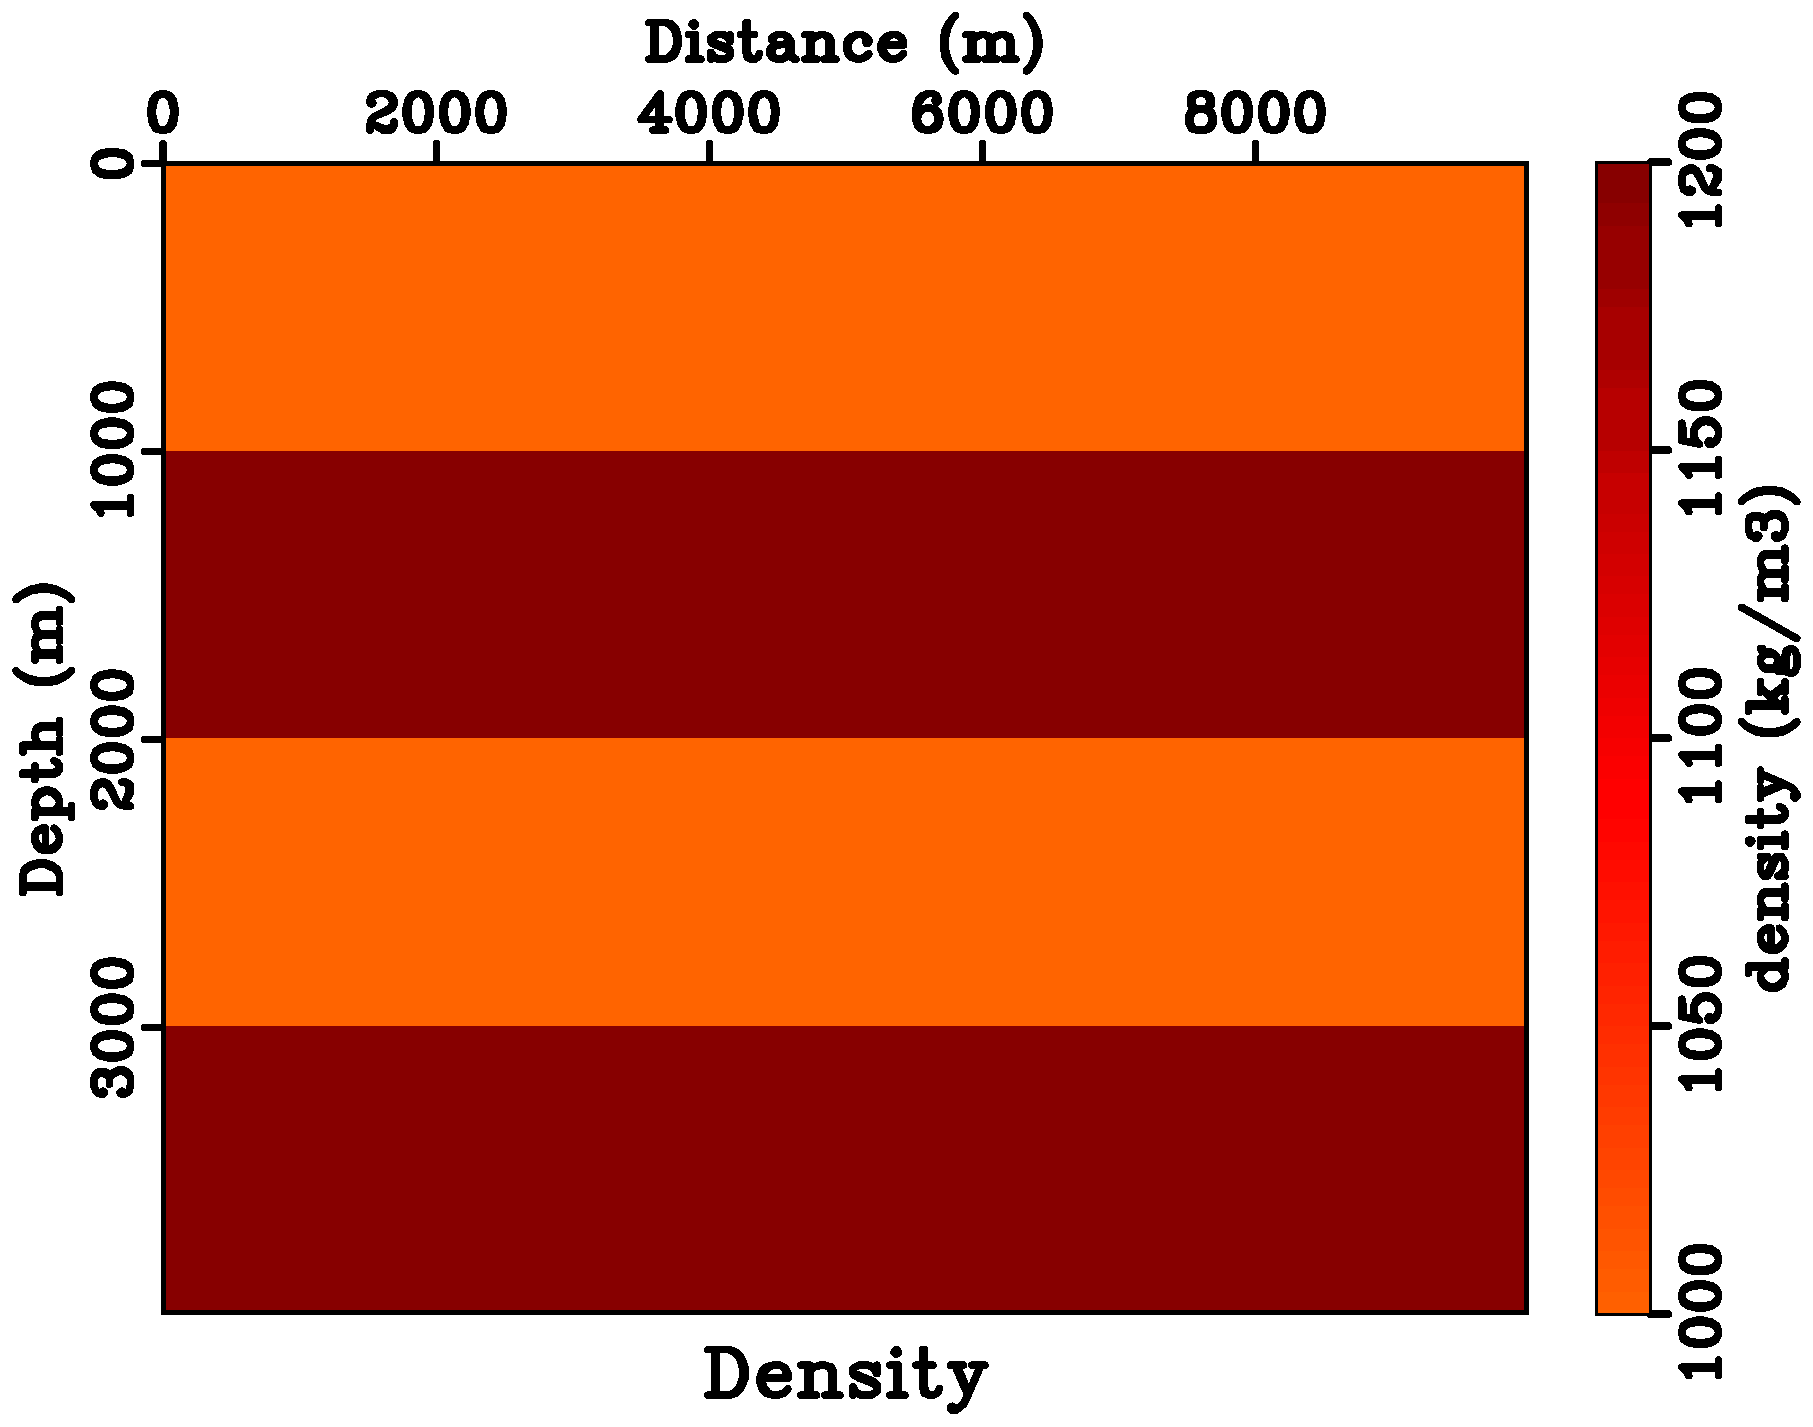
\epsfig{file=Fig/rho-1,width=10cm}
\end{figure}
\end{frame}
%-----------------------------------------
\begin{frame}{Numerical example}
%-----------------------------------------
%
\begin{figure}
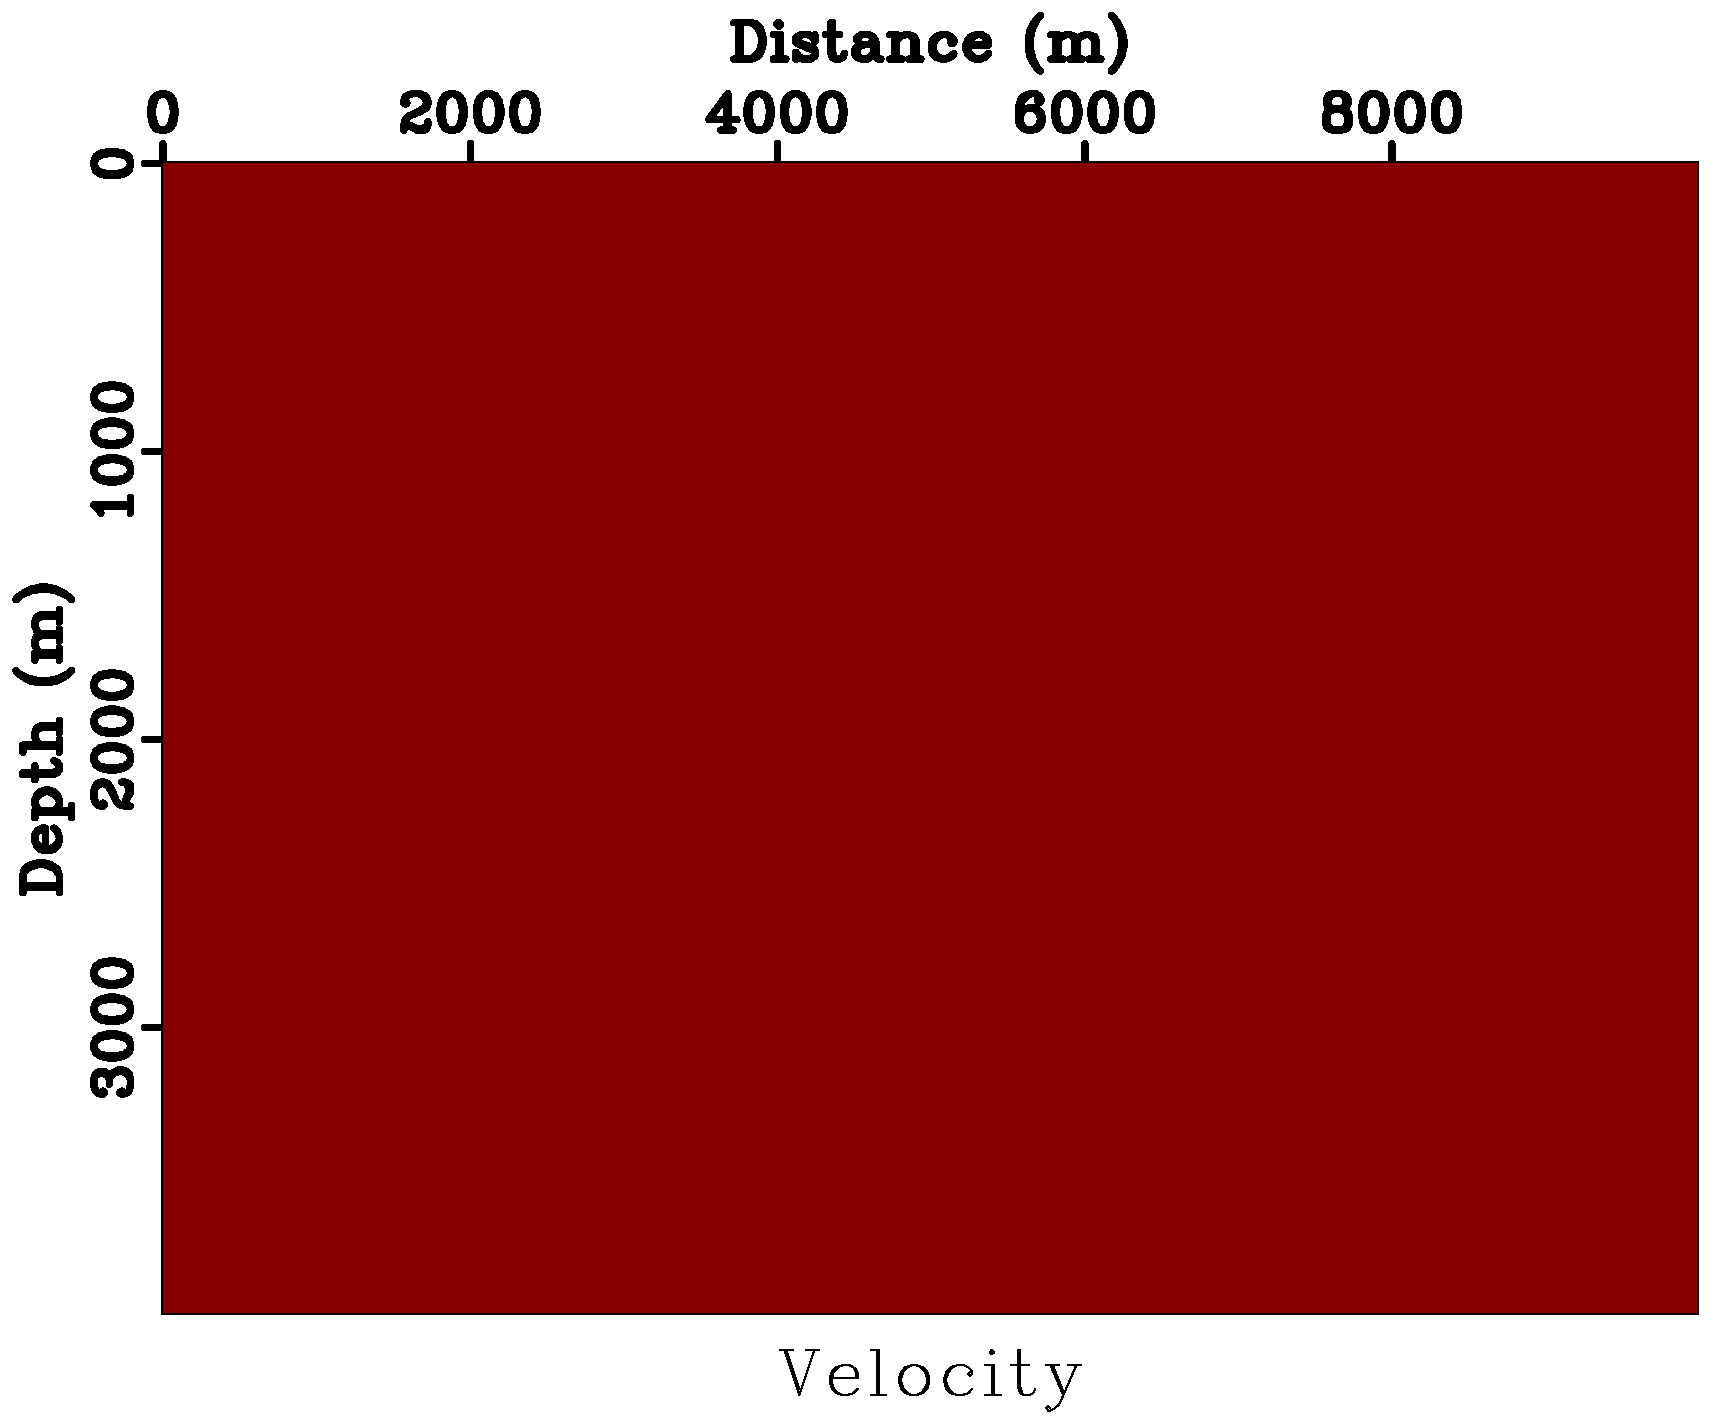
\epsfig{file=Fig/vp-1,width=10cm}
\end{figure}
\end{frame}
%-----------------------------------------
\begin{frame}{Numerical example}
%-----------------------------------------
%
\begin{figure}
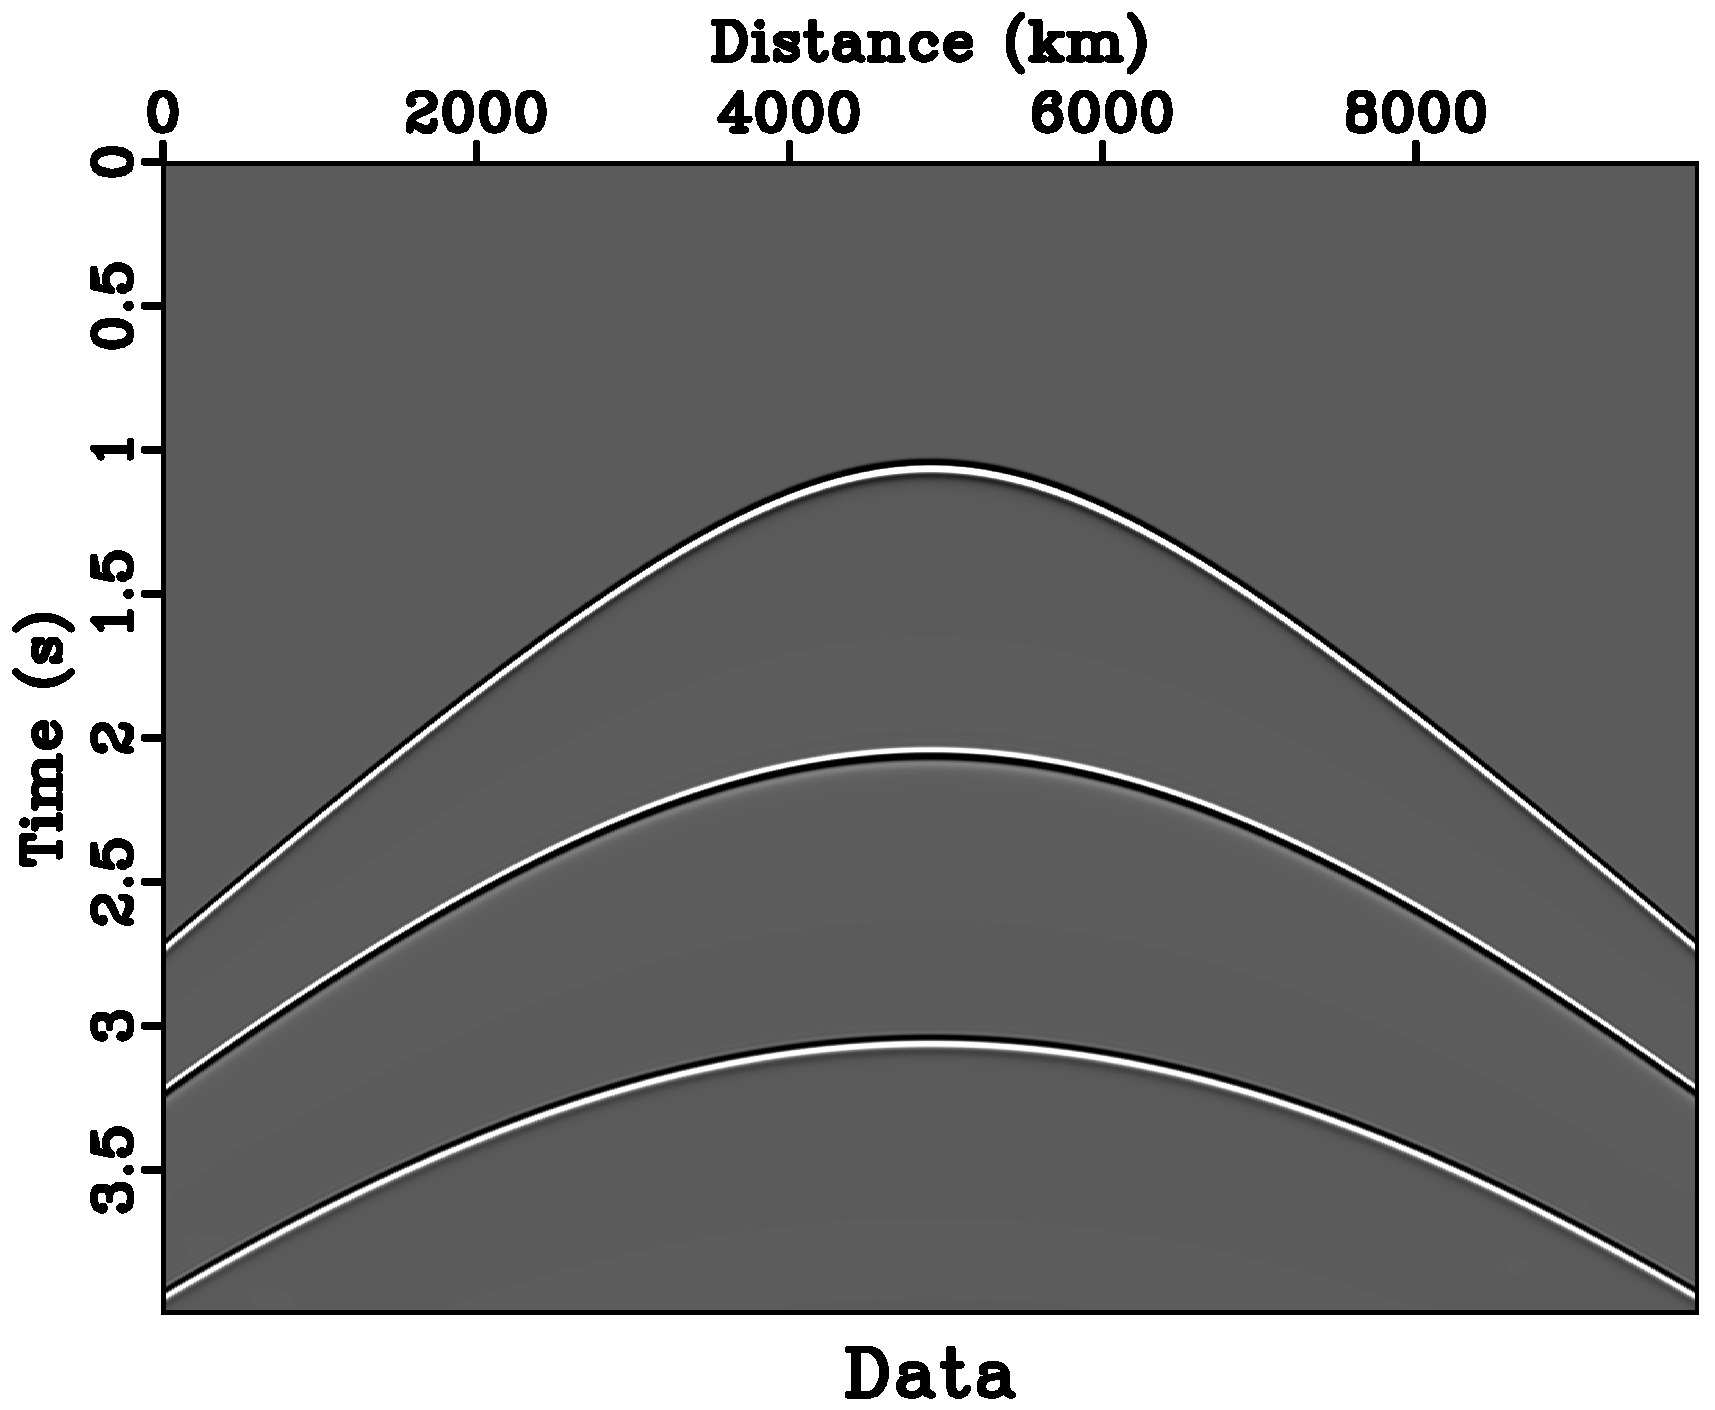
\epsfig{file=Fig/data-1-scatter,width=10cm}
\end{figure}
\end{frame}
%-----------------------------------------
\begin{frame}{Numerical example}
%-----------------------------------------
$p(\xx,\xx_s,t)$ at depth of 1000 m.
%
\begin{figure}
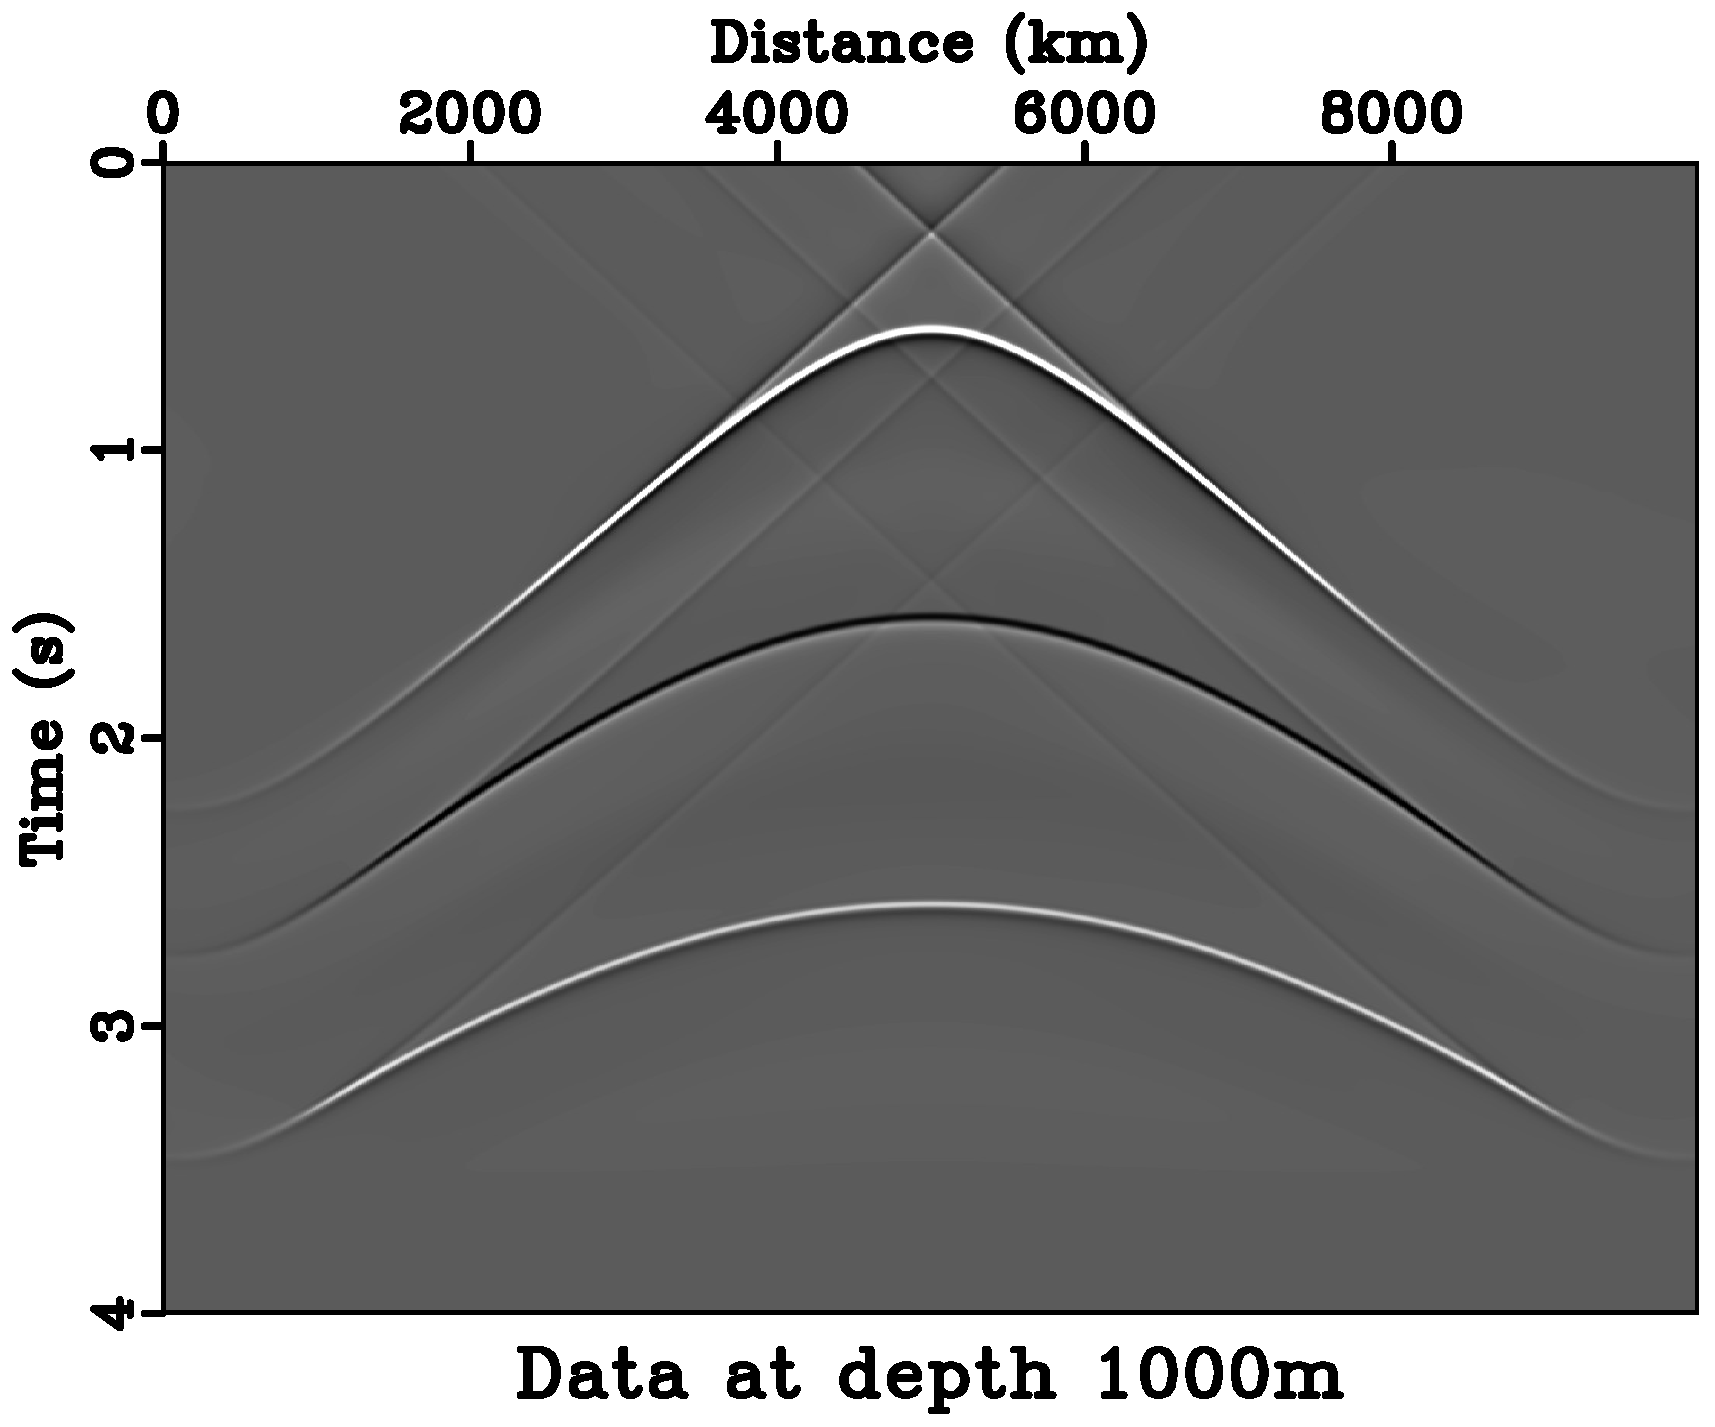
\epsfig{file=Fig/data-1-scatter-redat,width=8cm}
\end{figure}
\end{frame}
%-----------------------------------------
\begin{frame}{Imaging condition III}
%-----------------------------------------
\begin{figure}
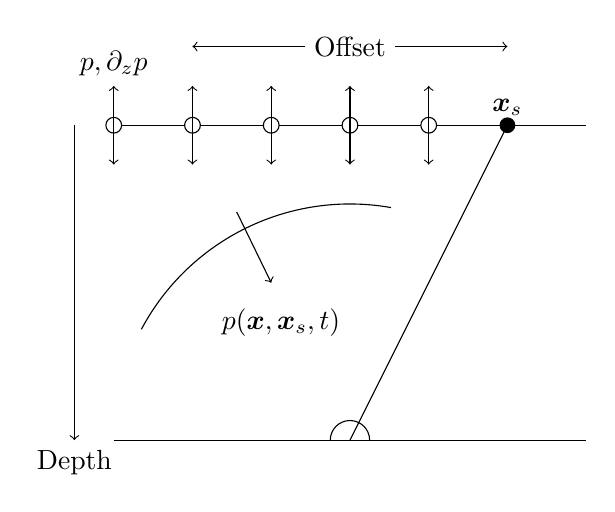
\begin{tikzpicture}[scale=1.0]
  \draw[->] (-0.5,4.0) -- (-0.5,0.0) node[below]{Depth} ;     %Draw Depth axis
  \draw[<->] (1.0,5.0) -- node[fill=white]{Offset} (5.0,5.0); %Draw offset axis 
  \draw (0.0,0.0) -- (6.0,0.0) ;  %Top boundary
  \draw (0.0,4.0) -- (6.0,4.0) ;  %Bottom boundary

  \fill (5.0,4.0) node[above]{$\xx_s$} circle (0.1) ; % Draw source

  \fill[white] (0.0,4.0) circle (0.1) ; %Draw receiver
  \draw (0.0,4.0) circle (0.1) ;
  \draw[->] (0.0,4.0) -- (0.0,4.5);
  \draw[->] (0.0,4.0) -- (0.0,3.5);
  \draw (0.0,4.5) node[above]{$p,\partial_z p$};
  

  \fill[white](1.0,4.0) circle (0.1) ;
  \draw (1.0,4.0) node[above]{} circle (0.1) ;
  \draw[->] (1.0,4.0) -- (1.0,4.5);
  \draw[->] (1.0,4.0) -- (1.0,3.5);

  \fill[white] (2.0,4.0) circle (0.1) ;
  \draw (2.0,4.0) circle (0.1) ;
  \draw[->] (2.0,4.0) -- (2.0,4.5);
  \draw[->] (2.0,4.0) -- (2.0,3.5);

  \fill[white] (3.0,4.0) circle (0.1) ;
  \draw (3.0,4.0) circle (0.1) ;
  \draw[->] (3.0,4.0) -- (3.0,4.5);
  \draw[->] (3.0,4.0) -- (3.0,3.5);

  \fill[white] (4.0,4.0) circle (0.1) ;
  \draw (4.0,4.0) circle (0.1) ;
  \draw[->] (4.0,4.0) -- (4.0,4.5);
  \draw[->] (4.0,4.0) -- (4.0,3.5);

  \draw[<-] (2,2)-- +(116:1);
  \draw (3,0) +(0:0.25) arc(0:180:0.25);
  \draw (3,0) +(80:3) arc(80:152:3);
  \draw (3.0,1.5) node[left]{$p(\xx,\xx_s,t)$};


  \draw (5.0,4.0) -- (3.0,0.0) ;
  %\draw (3.0,0.0) -- (1.0,4.0) ;
\end{tikzpicture}
%\label{fig:si-1}

$p$: Scattered wavefield \\
$\xx_s$: Source position\\
$\xx,t$: Position,time
\end{figure}
\end{frame}
%-----------------------------------------
\begin{frame}{Imaging condition IV}
%-----------------------------------------
\begin{figure}
\begin{tikzpicture}[scale=1.0]
  \draw[->] (-0.5,4.0) -- (-0.5,0.0) node[below]{Depth} ;     %Draw Depth axis
  \draw[<->] (1.0,5.0) -- node[fill=white]{Offset} (5.0,5.0); %Draw offset axis 
  \draw (0.0,0.0) -- (6.0,0.0) ;  %Top boundary
  \draw (0.0,4.0) -- (6.0,4.0) ;  %Bottom boundary

  \fill (5.0,4.0) node[above]{$\xx_s$} circle (0.1) ; % Draw source

  \fill[white] (0.0,0.5) circle (0.1) ; %Draw receiver
  \draw (0.0,0.5) circle (0.1) ;
  

  \fill[white](1.0,0.5) circle (0.1) ;
  \draw (1.0,0.5) node[above]{} circle (0.1) ;

  \fill[white] (2.0,0.5) circle (0.1) ;
  \draw (2.0,0.5) circle (0.1) ;

%  \fill[white] (3.0,0.5) circle (0.1) ;
%  \draw (3.0,0.5) circle (0.1) ;

%  \fill[white] (4.0,0.5) circle (0.1) ;
%  \draw (4.0,0.5) circle (0.1) ;

  \draw[->] (3,0)-- (0.0,0.5);
  \draw[->] (3,0)-- (1.0,0.5);
  \draw[->] (3,0)-- (2.0,0.5);
  %\draw[->] (3,0)-- (3.0,0.5);
  %\draw[->] (3,0)-- (4.0,0.5);
%  \draw (3,0) +(0:0.25) arc(0:180:0.25);
%  \draw (3,0) +(80:3) arc(80:152:3);
  \draw (3.0,1.5) node[left]{$p(\xx,\xx_s,t)$};


  \draw (5.0,4.0) -- (3.0,0.0) ;
  %\draw (3.0,0.0) -- (1.0,4.0) ;
\end{tikzpicture}
%\label{fig:si-1}
\end{figure}
\end{frame}
%-----------------------------------------
\begin{frame}{Imaging condition V}
%-----------------------------------------
\begin{figure}
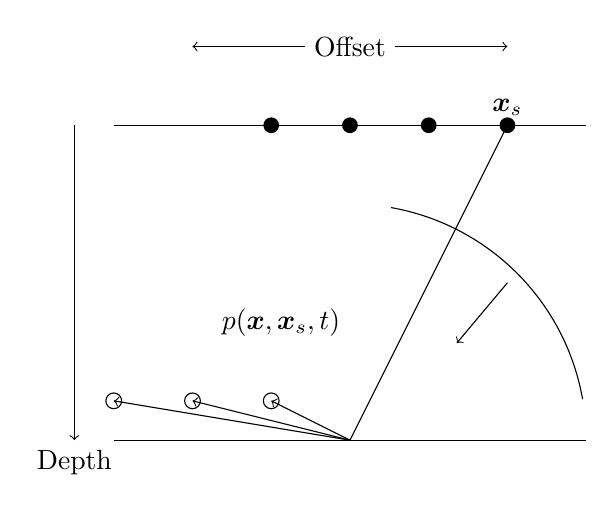
\begin{tikzpicture}[scale=1.0]
  \draw[->] (-0.5,4.0) -- (-0.5,0.0) node[below]{Depth} ;     %Draw Depth axis
  \draw[<->] (1.0,5.0) -- node[fill=white]{Offset} (5.0,5.0); %Draw offset axis 
  \draw (0.0,0.0) -- (6.0,0.0) ;  %Top boundary
  \draw (0.0,4.0) -- (6.0,4.0) ;  %Bottom boundary

  \fill (5.0,4.0) node[above]{$\xx_s$} circle (0.1) ; % Draw source
  \fill (4.0,4.0) node[above]{} circle (0.1) ; % Draw source
  \fill (3.0,4.0) node[above]{} circle (0.1) ; % Draw source
  \fill (2.0,4.0) node[above]{} circle (0.1) ; % Draw source

  \fill[white] (0.0,0.5) circle (0.1) ; %Draw receiver
  \draw (0.0,0.5) circle (0.1) ;
  

  \fill[white](1.0,0.5) circle (0.1) ;
  \draw (1.0,0.5) node[above]{} circle (0.1) ;

  \fill[white] (2.0,0.5) circle (0.1) ;
  \draw (2.0,0.5) circle (0.1) ;

%  \fill[white] (3.0,0.5) circle (0.1) ;
%  \draw (3.0,0.5) circle (0.1) ;

%  \fill[white] (4.0,0.5) circle (0.1) ;
%  \draw (4.0,0.5) circle (0.1) ;

  \draw[->] (3,0)-- (0.0,0.5);
  \draw[->] (3,0)-- (1.0,0.5);
  \draw[->] (3,0)-- (2.0,0.5);
%  \draw[->] (3,0)-- (3.0,0.5);
%  \draw[->] (3,0)-- (4.0,0.5);
%  \draw (3,0) +(0:0.25) arc(0:180:0.25);
%  \draw (3,0) +(80:3) arc(80:152:3);
  \draw (3.0,1.5) node[left]{$p(\xx,\xx_s,t)$};
\draw (3,0) +(80:3) arc(80:10:3);

  \draw[->] (5,2)-- +(230:1);

  \draw (5.0,4.0) -- (3.0,0.0) ;
  %\draw (3.0,0.0) -- (1.0,4.0) ;
\end{tikzpicture}
%\label{fig:si-1}
\end{figure}
\end{frame}
%-----------------------------------------
\begin{frame}{Imaging condition VI}
%-----------------------------------------
\begin{figure}
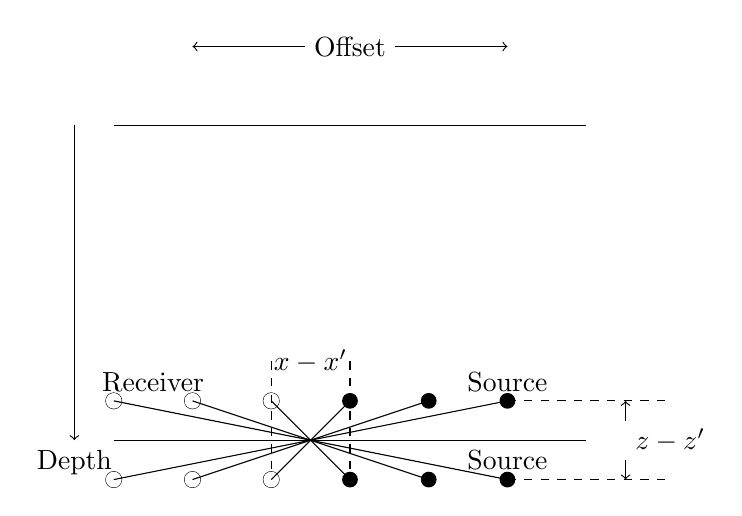
\begin{tikzpicture}[scale=1.0]
   \draw[->] (-0.5,4.0) -- (-0.5,0.0) node[below]{Depth} ;      %Depth axis 
   \draw[<->] (1.0,5.0) -- node[fill=white]{Offset} (5.0,5.0);  %Offset axis  
  \draw (0.0,4.0) -- (6.0,4.0) ;                               % Boundary at top
  \draw (0.0,0.0) -- (6.0,0.0) ;                               % Boundary at depth

  \fill (3.0,0.5) node[above]{} circle (0.1) ;           % Draw source
  \fill (4.0,0.5) node[above]{} circle (0.1) ;           % Draw source
  \fill (5.0,0.5) node[above]{Source} circle (0.1) ;     % Draw source text

  \draw (2.0,0.5) circle (0.1) ;             %Draw receiver
  \fill[white] (2.0,0.5) circle (0.1) ;

  \draw (1.0,0.5) circle (0.1) ;             %Draw receiver
  \fill[white] (1.0,0.5) circle (0.1) ;

  \draw (0.0,0.5) circle (0.1) ;             %Draw receiver
  \fill[white] (0.0,0.5) circle (0.1) ;
  \draw (0.5,0.5) node[above]{Receiver} ;    %Draw receiver text 

  \draw (3.0,0.5) -- (2.5,0.0);              % Draw ray from source to midpoint
  \draw (4.0,0.5) -- (2.5,0.0);              % Draw ray from source to midpoint
  \draw (5.0,0.5) -- (2.5,0.0);              % Draw ray from source to midpoint

  \draw (2.0,0.5) -- (2.5,0.0);              % Draw ray from receiver to midpoint
  \draw (1.0,0.5) -- (2.5,0.0);              % Draw ray from receiver to midpoint
  \draw (0.0,0.5) -- (2.5,0.0);              % Draw ray from receiver to midpoint

  \draw[dashed] (2.0,1.0) -- (2.0,-0.5);     %Draw vertical dashed line
  \draw[dashed] (3.0,1.0) -- (3.0,-0.5);     %Draw vertical dashed line
  \draw (2.5,1.0) node {$x-x'$};           % Draw equation
  \draw[dashed] (5.0,0.5) -- (7.0,0.5);     %Draw vertical dashed line
  \draw[dashed] (5.0,-0.5) -- (7.0,-0.5);     %Draw vertical dashed line
  \draw (6.5,0.0) node[right]{$z-z'$};           % Draw equation
  \draw[->] (6.5,0.25) -- (6.5,0.5);
  \draw[->] (6.5,-0.25) -- (6.5,-0.5);



  \fill (3.0,-0.5) node[above]{} circle (0.1) ;           % Draw source
  \fill (4.0,-0.5) node[above]{} circle (0.1) ;           % Draw source
  \fill (5.0,-0.5) node[above]{Source} circle (0.1) ;     % Draw source text

  \draw (2.0,-0.5) circle (0.1) ;             %Draw receiver
  \fill[white] (2.0,-0.5) circle (0.1) ;

  \draw (1.0,-0.5) circle (0.1) ;             %Draw receiver
  \fill[white] (1.0,-0.5) circle (0.1) ;

  \draw (0.0,-0.5) circle (0.1) ;             %Draw receiver
  \fill[white] (0.0,-0.5) circle (0.1) ;
  %\draw (0.5,0.5) node[above]{Receiver} ;    %Draw receiver text 

  \draw (3.0,-0.5) -- (2.5,0.0);              % Draw ray from source to midpoint
  \draw (4.0,-0.5) -- (2.5,0.0);              % Draw ray from source to midpoint
  \draw (5.0,-0.5) -- (2.5,0.0);              % Draw ray from source to midpoint

  \draw (2.0,-0.5) -- (2.5,0.0);              % Draw ray from receiver to midpoint
  \draw (1.0,-0.5) -- (2.5,0.0);              % Draw ray from receiver to midpoint
  \draw (0.0,-0.5) -- (2.5,0.0);              % Draw ray from receiver to midpoint
\end{tikzpicture}
\end{figure}

$x-x'$: Horizontal offset \\
$z-z'$: Vertical offset 
\end{frame}
%-----------------------------------------
\begin{frame}{Imaging}
%-----------------------------------------
\begin{eqnarray}
 p(\xx,\xx_s,-t)*h(t)-p(\xx,\xx_s,t)*h(-t) =\nonumber\\
\int dS(\xx')\, \left[p(\xx',\xx_s,-t)*\nabla p(\xx,\xx',t)\right.\nonumber\\
   -\left. p(\xx,\xx',t)*\nabla p(\xx',\xx_s,-t)\right]\cdot \nn(\xx')
&&                   \label{eq:9000}
\end{eqnarray}
Use reciprocity again
\begin{eqnarray}
 p(\xx_s,\xx,-t)*h(t)-p(\xx_s,\xx,t)*h(-t) =\nonumber\\
\int dS(\xx')\, \left[p(\xx_s,\xx',-t)*\nabla p(\xx,\xx',t)\right.\nonumber\\
   -\left. p(\xx,\xx',t)*\nabla p(\xx_s,\xx',-t)\right]\cdot \nn(\xx')
&&                   \label{eq:9100}
\end{eqnarray}
\end{frame}
%-----------------------------------------
\begin{frame}{Imaging}
%-----------------------------------------
Rename $\xx_s$ to $\xx'$ and vice versa
\begin{eqnarray}
 p(\xx',\xx,-t)*h(t)-p(\xx',\xx,t)*h(-t) =\nonumber\\
\int dS(\xx_s)\, \left[p(\xx',\xx_s,-t)*\nabla p(\xx,\xx_s,t)\right.\nonumber\\
   -\left. p(\xx,\xx_s,t)*\nabla p(\xx',\xx_s,-t)\right]\cdot \nn(\xx')
&&                   \label{eq:9200}
\end{eqnarray}
\end{frame}

%-----------------------------------------
\begin{frame}{Interferometry}
%-----------------------------------------
\begin{figure}
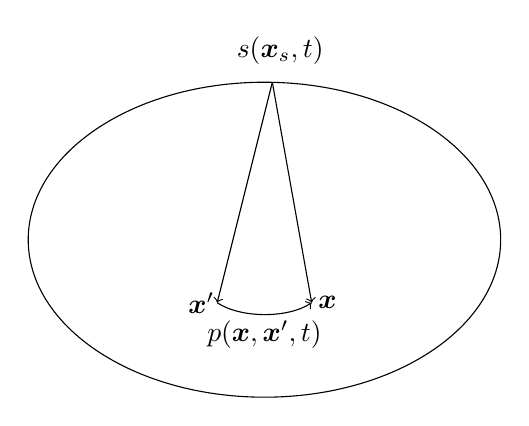
\begin{tikzpicture}
\draw (0,0) ellipse (3cm and 2cm);
\draw (0.2,2.4) node {$s(\xx_s,t)$};
\draw (-0.8,-0.8) node {$\xx'$};
\draw[->] (0.1,2.0) -- (-0.6,-0.8);
\draw (0.8,-0.8) node {$\xx$};
\draw[->] (0.1,2.0) -- (0.6,-0.8);
\draw[->] (-0.6,-0.8) .. controls (-0.3,-1.0)  and (0.3,-1.0) .. (0.6,-0.8);
\draw (-0.0,-1.2) node {$p(\xx,\xx',t)$};
\end{tikzpicture}
\end{figure}
\end{frame}
%-----------------------------------------
\begin{frame}{Imaging}
%-----------------------------------------
Define $r(\xx',\xx,t) = p(\xx',\xx,-t)*h(t)-p(\xx',\xx,t)*h(-t)$
\begin{eqnarray}
 r(\xx',\xx,t)=\nonumber\\
\int dS(\xx_s)\, \int d\tau\, \left[p(\xx',\xx_s,t+\tau)\nabla p_0(\xx,\xx_s,\tau)\right.\nonumber\\
   -\left. p_0(\xx,\xx_s,t+\tau)\nabla p(\xx',\xx_s,\tau)\right]\cdot \nn(\xx')
&&                   \label{eq:9300}
\end{eqnarray}
\begin{eqnarray}
 r(\xx',\xx,t=0)=\nonumber\\
\int dS(\xx_s)\, \int d\tau\, \left[p(\xx',\xx_s,\tau)\nabla p_0(\xx,\xx_s,\tau)\right.\nonumber\\
   -\left. p_0(\xx,\xx_s,\tau)\nabla p(\xx',\xx_s,\tau)\right]\cdot \nn(\xx')
&&                   \label{eq:9400}
\end{eqnarray}
$p_0$: Forward wavefield 
\end{frame}
%-----------------------------------------
\begin{frame}{Imaging}
%-----------------------------------------
The final imaging formula can be interpreted as
\begin{enumerate}
\item The left hand side is the wavefield at position $\xx'$ due to a source at position $\xx$.
      These two positions are arbitrary, so the sources (and receivers) are virtual.
\item The two terms on the right hand side is the cross-correlation between the extrapolated data
      and forward modelled data. Both the pressure and the derivative of the pressure are needed as
      data.
\end{enumerate}
\end{frame}
%-----------------------------------------
\begin{frame}{Imaging}
%-----------------------------------------
Migration consists in:
\begin{enumerate}
\item Compute the forward wavefield $p(\xx,\xx_s,t)$
      from equation \eqref{eq:fmod}
\item Compute the backward wavefield $p(\xx',\xx_s,t)$ from equation \eqref{eq:fback}.
\item Compute the image from equation \eqref{eq:9400}
\end{enumerate}
\end{frame}
%---------------------------------
\begin{frame}{Simplification}
%---------------------------------
\begin{eqnarray}
 r(\xx',\xx,t=0)=\nonumber\\
\int dS(\xx_s)\, \int d\tau\, \left[p(\xx',\xx_s,\tau)\nabla p_0(\xx,\xx_s,\tau)\right.\nonumber\\
   -\left. p_0(\xx,\xx_s,\tau)\nabla p(\xx',\xx_s,\tau)\right]\cdot \nn(\xx')
&&                   \label{eq:10400}
\end{eqnarray}
Horizontal receiver implies
\begin{eqnarray}
 r(\xx',\xx,t=0)=\nonumber\\
\int dS(\xx_s)\, \int d\tau\, \left[p(\xx',\xx_s,\tau)\partial_z p_0(\xx,\xx_s,\tau)\right.\nonumber\\
   -\left. p_0(\xx,\xx_s,\tau)\partial_z' p(\xx',\xx_s,\tau)\right]
&&                   \label{eq:10500}
\end{eqnarray}
\end{frame}
%---------------------------------
\begin{frame}{Simplification}
%---------------------------------
$\partial_z p(\xx',\xx_s.t)=0$ (No recorded pressure gradient)
\begin{eqnarray}
 r(\xx',\xx,t=0)=
\int dS(\xx_s)\, \int d\tau\, p(\xx',\xx_s,\tau)\partial_z p_0(\xx,\xx_s,\tau)\nonumber\\
&&                   \label{eq:10600}
\end{eqnarray}
\end{frame}
%-----------------------------------------
\begin{frame}{Classical Imaging condition}
%-----------------------------------------
For $\xx'=\xx$ and by ignoring $\partial_z$ this is the classical imaging condition (Claerbout, 1971)
\begin{eqnarray}
  r_{c}(\xx) =
    \sum_{\xx_s}\sum_{\tau}p_0(\xx,\xx_s,\tau)p(\xx,\xx_s,\tau)\nonumber\\ 
                                                 \nonumber
\end{eqnarray}
Ignoring $\partial_z$ implies an unfocused image with
less than optimal resolution and incorrect amplitudes.
\end{frame}
%------------------------------------------------------
\begin{frame}{Numerical examples}
%------------------------------------------------------
Common image point gather (CIP) in the center of the model
Classical imaging condition:
\begin{figure}
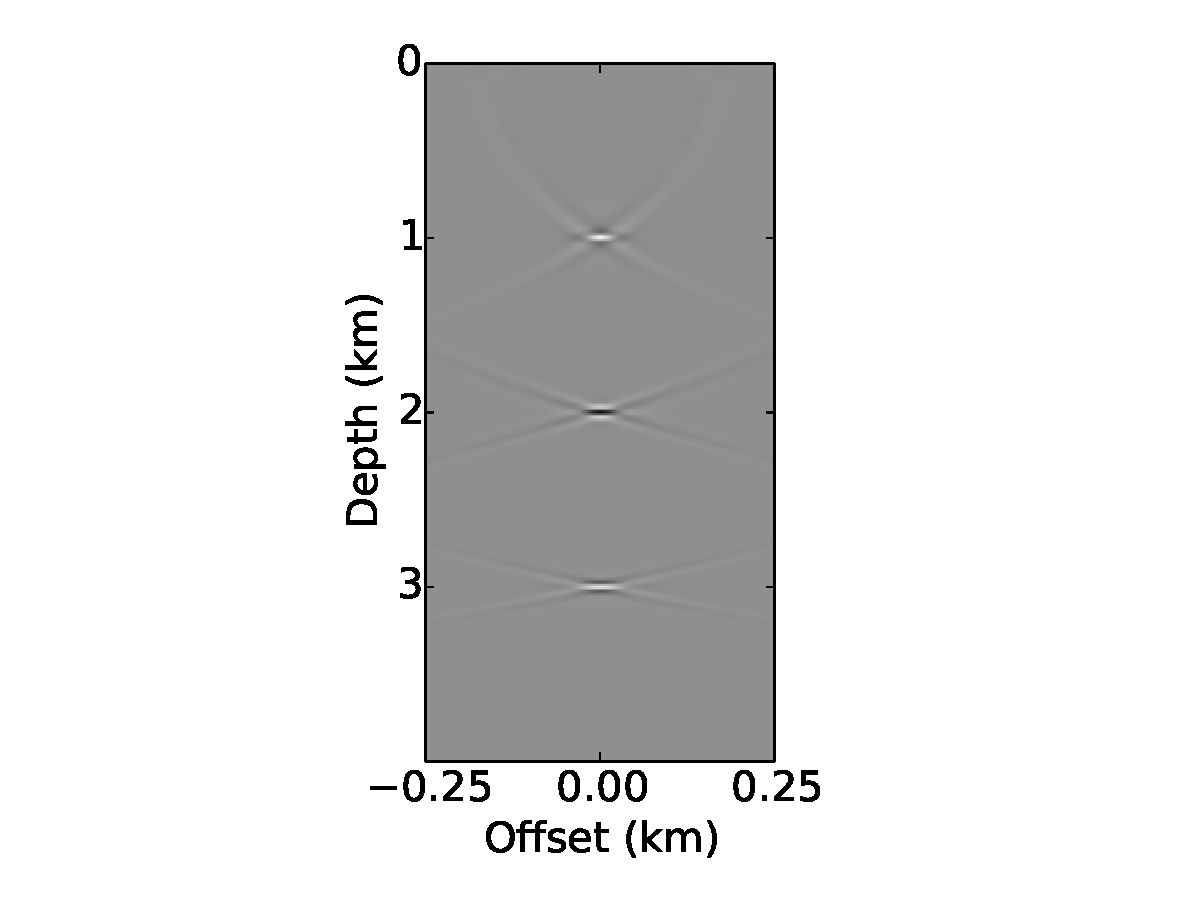
\epsfig{file=Fig/case-1-cig,width=9cm}
\end{figure}
\end{frame}
%------------------------------------------------------
\begin{frame}{Numerical examples}
%------------------------------------------------------
Horizontal profile through reflector at 1000m depth
\begin{figure}
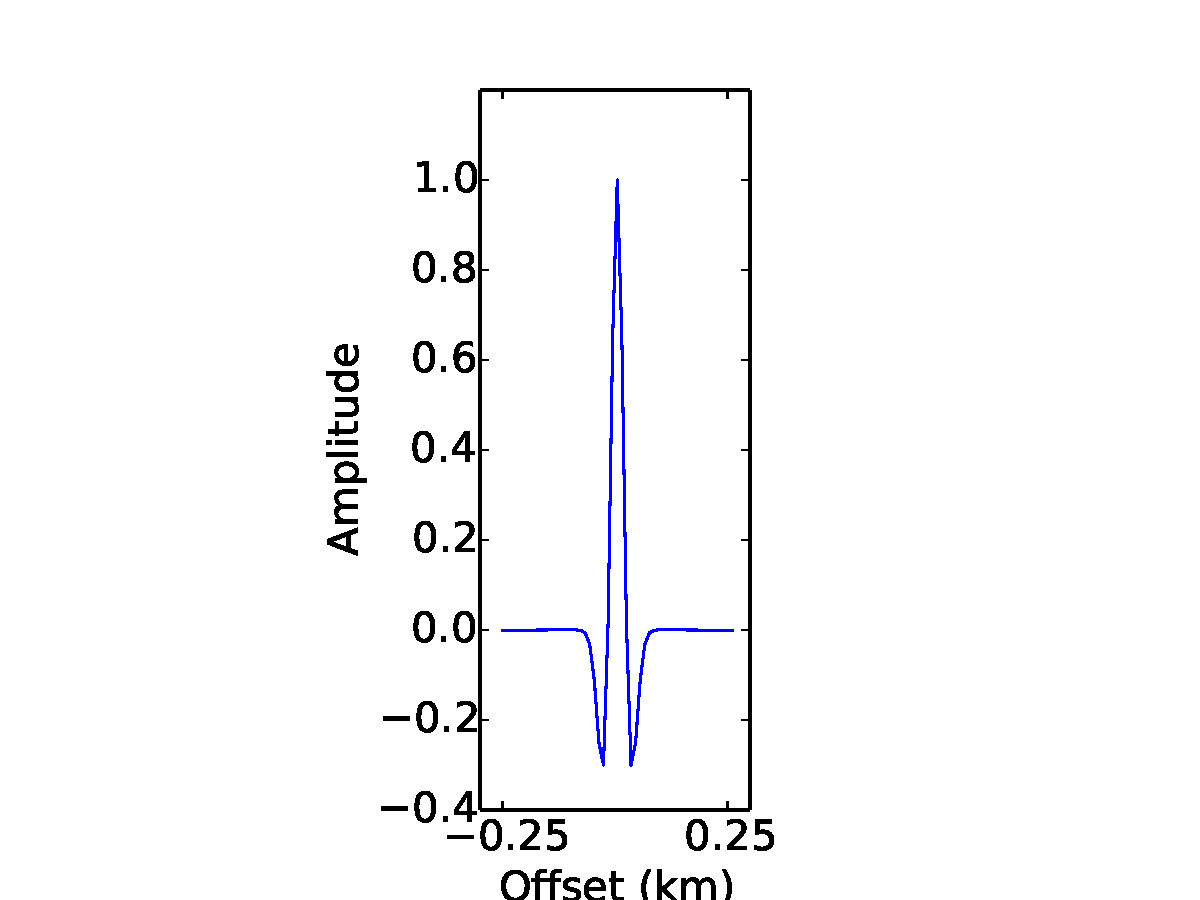
\epsfig{file=Fig/case-1-cig-h,width=9cm}
\end{figure}
\end{frame}
%------------------------------------------------------
\begin{frame}{Numerical examples}
%------------------------------------------------------
Common image point gather (CIP) in the center of the model.\\
New imaging condition:
\begin{figure}
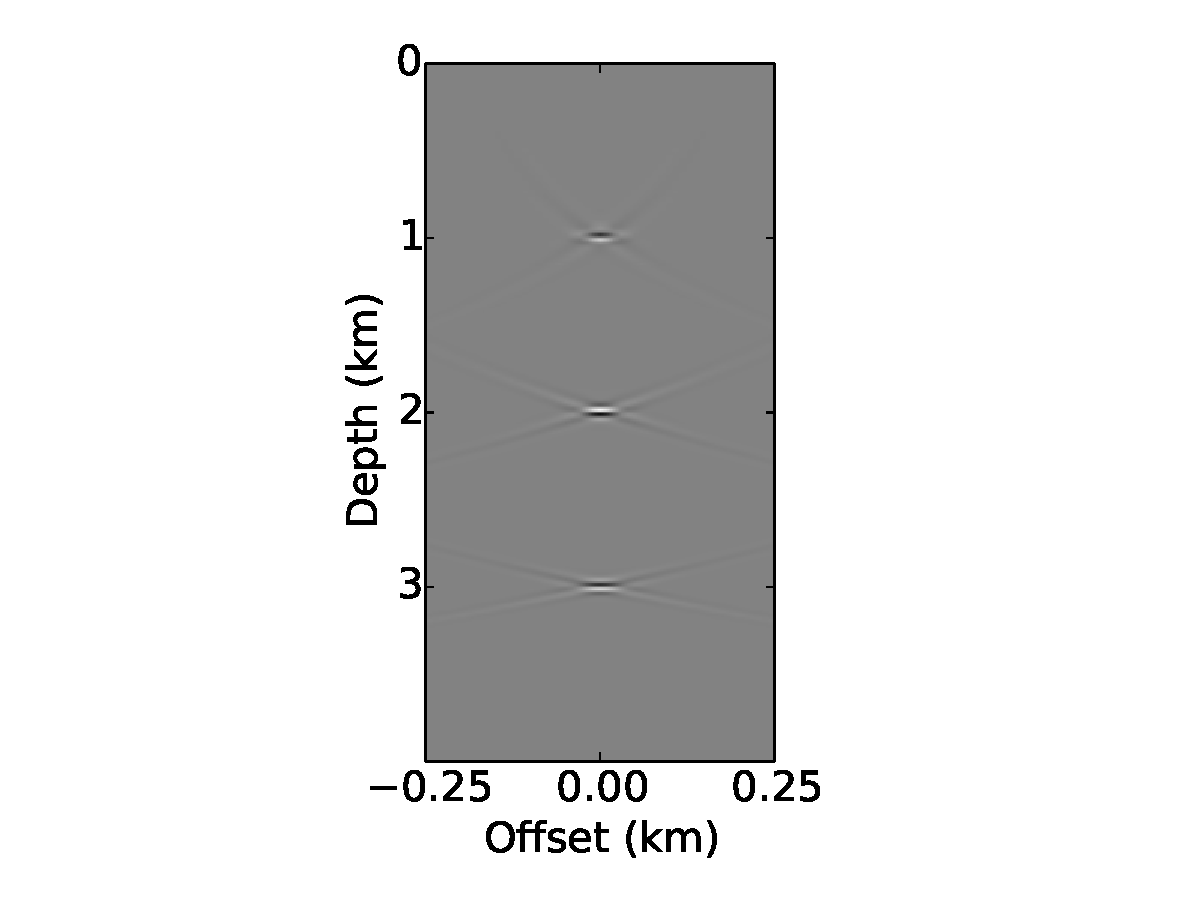
\epsfig{file=Fig/case-2-cig,width=9cm}
\end{figure}
\end{frame}
%------------------------------------------------------
\begin{frame}{Numerical examples}
%------------------------------------------------------
Horizontal profile through reflector at 1000m depth
\begin{figure}
%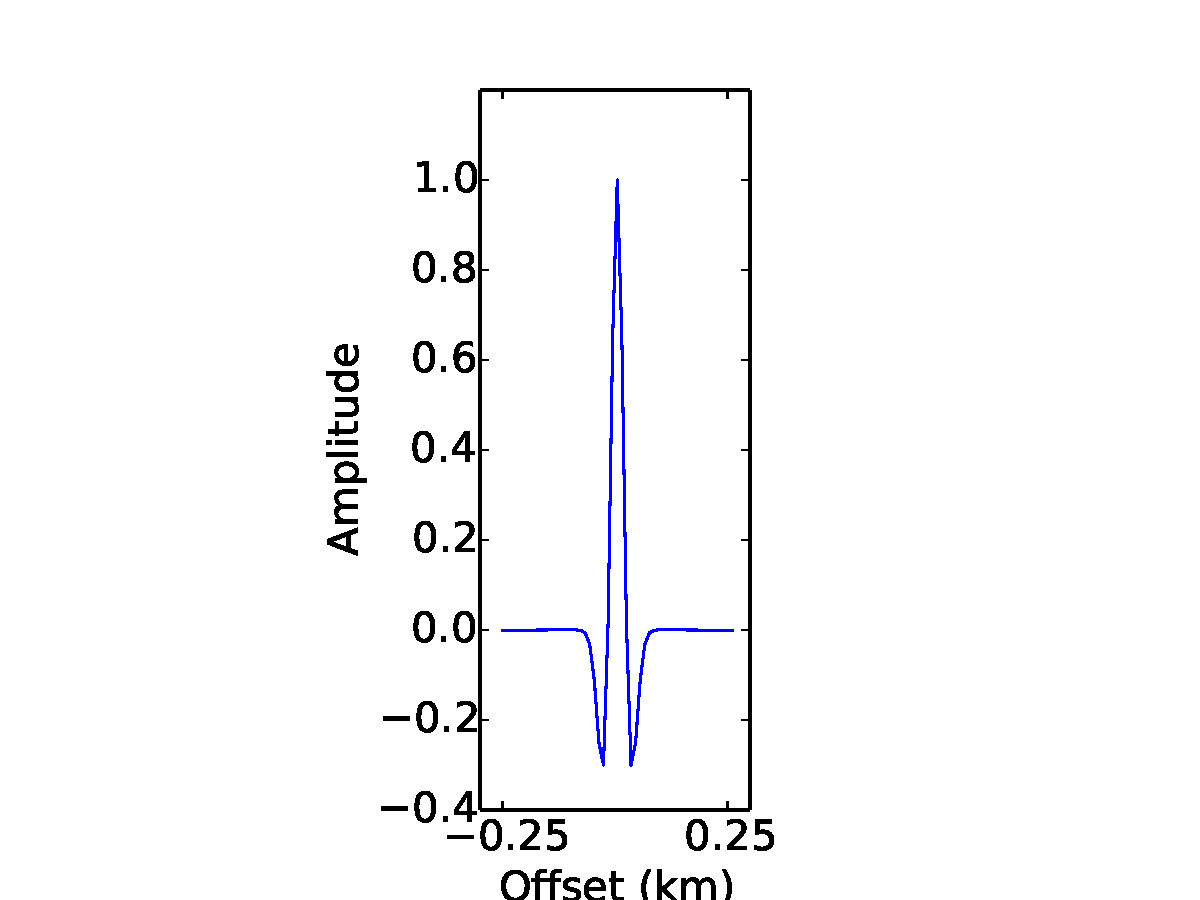
\epsfig{file=Fig/case-1-cig-h,width=9cm}
%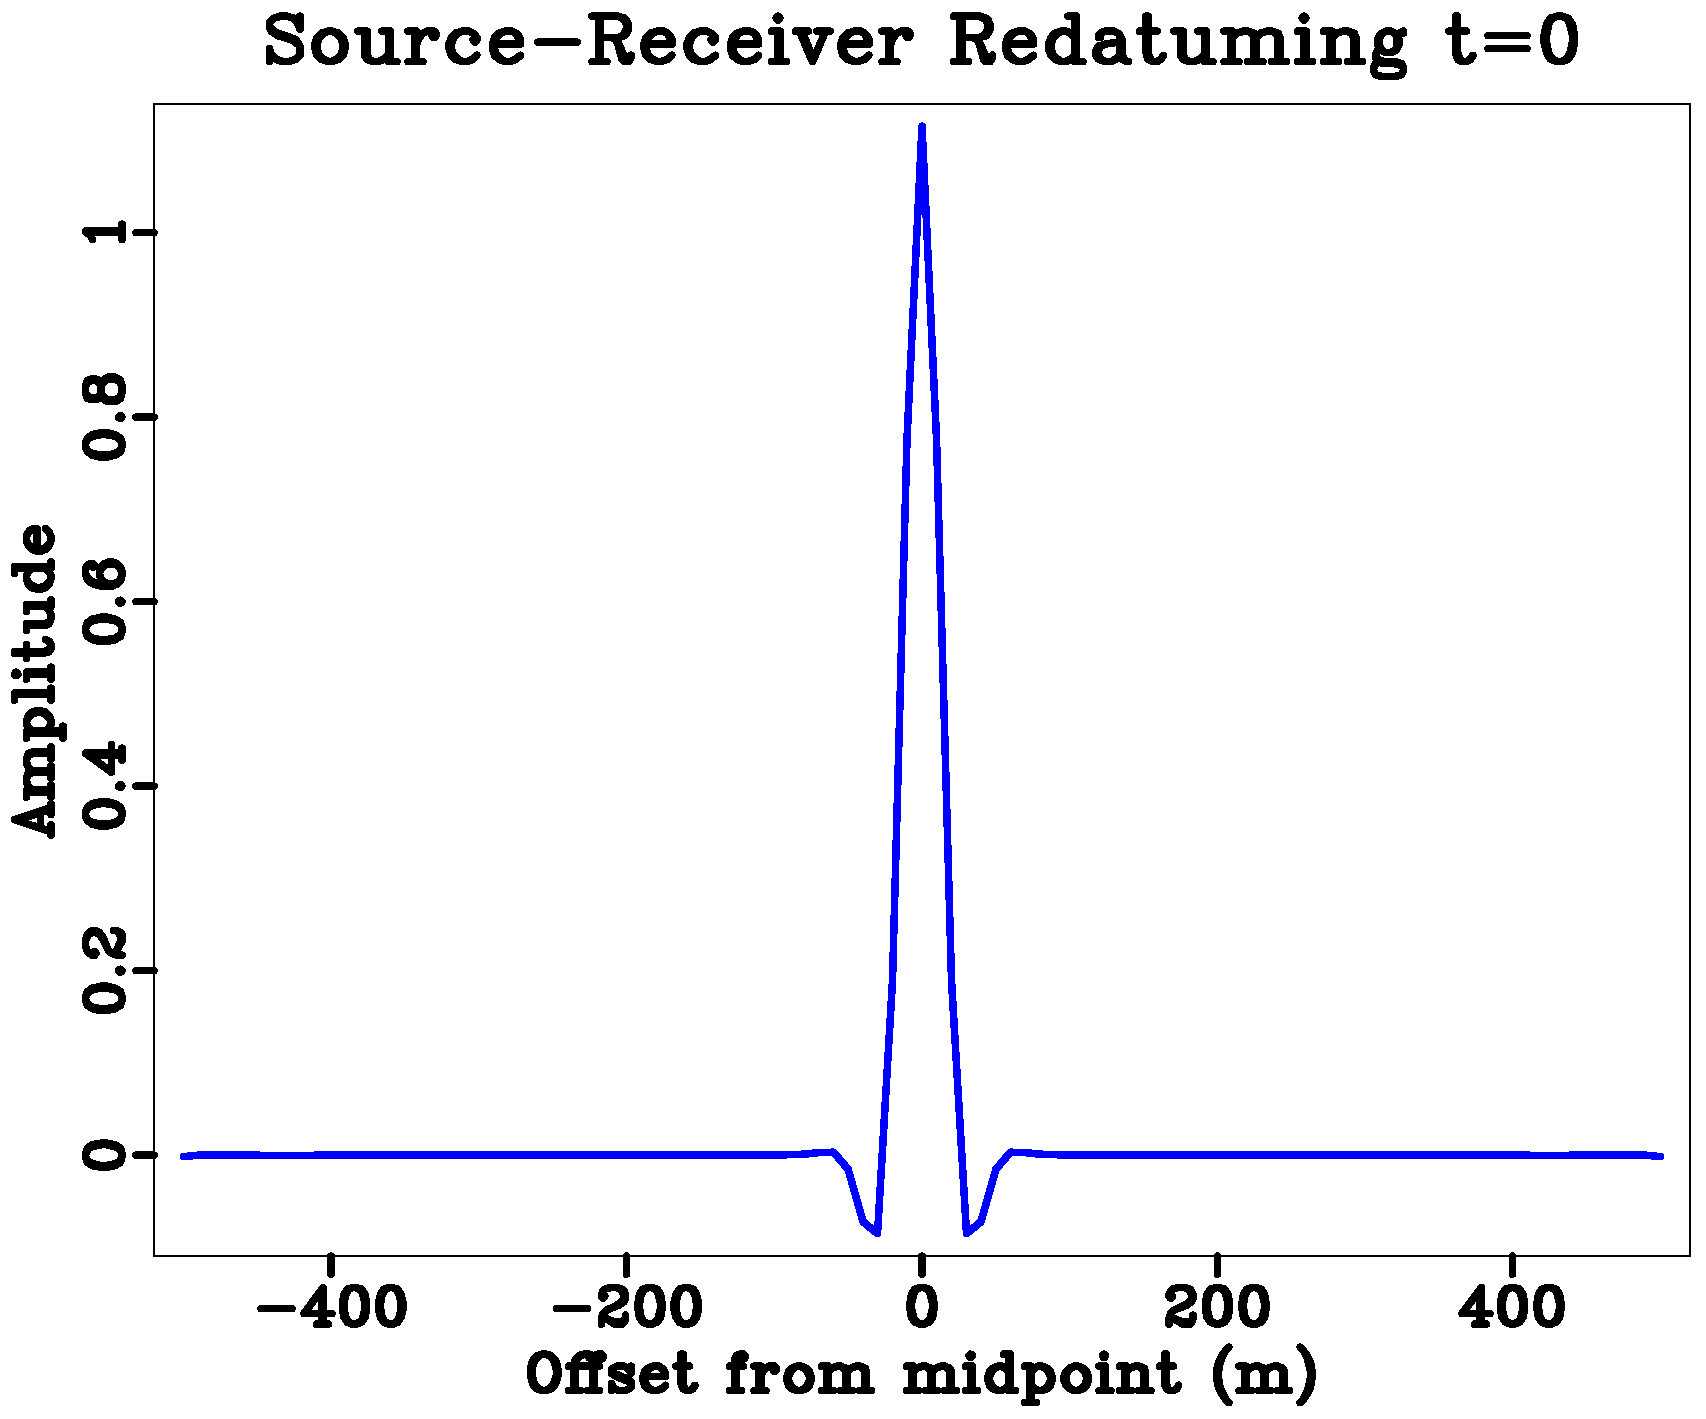
\epsfig{file=Fig/cip-1-ta-h-r1.pdf,width=9cm}
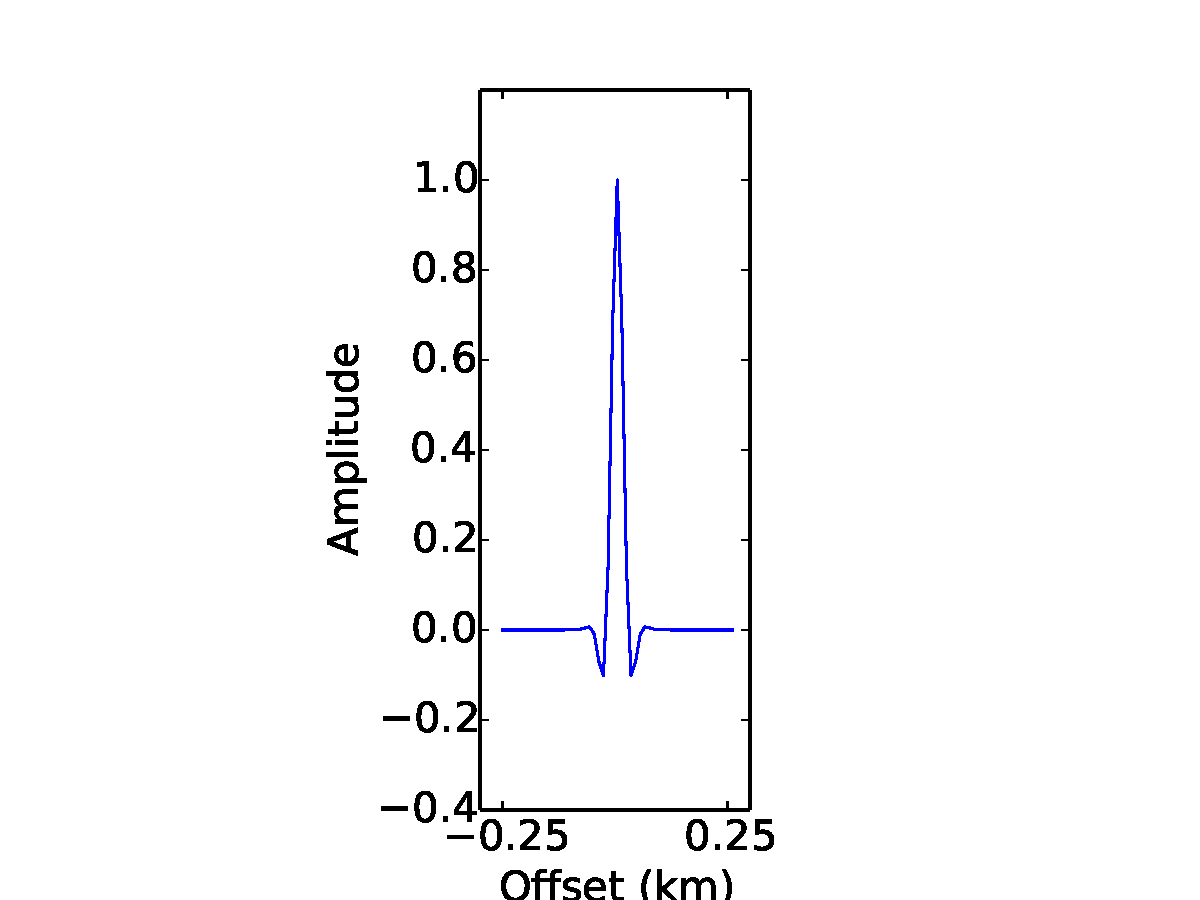
\epsfig{file=Fig/case-2-cig-h,width=9cm}
\end{figure}
\end{frame}
%------------------------------------------------------
\begin{frame}{Numerical example}
%------------------------------------------------------
Conventional imaging condition:
\begin{figure}
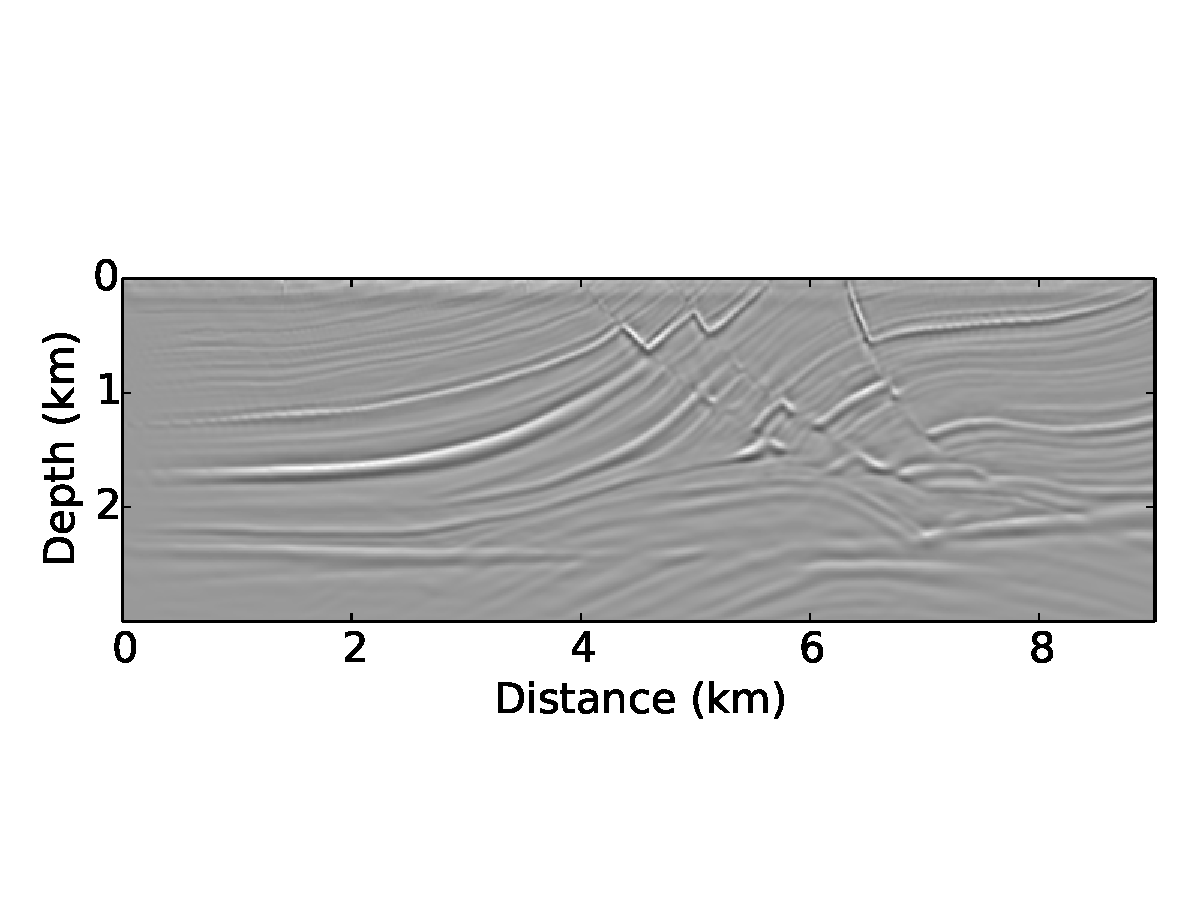
\epsfig{file=Fig/case-4-stack,width=10cm}
\end{figure}
\end{frame}
%------------------------------------------------------
\begin{frame}{Numerical example}
%------------------------------------------------------
New imaging condition:
\begin{figure}
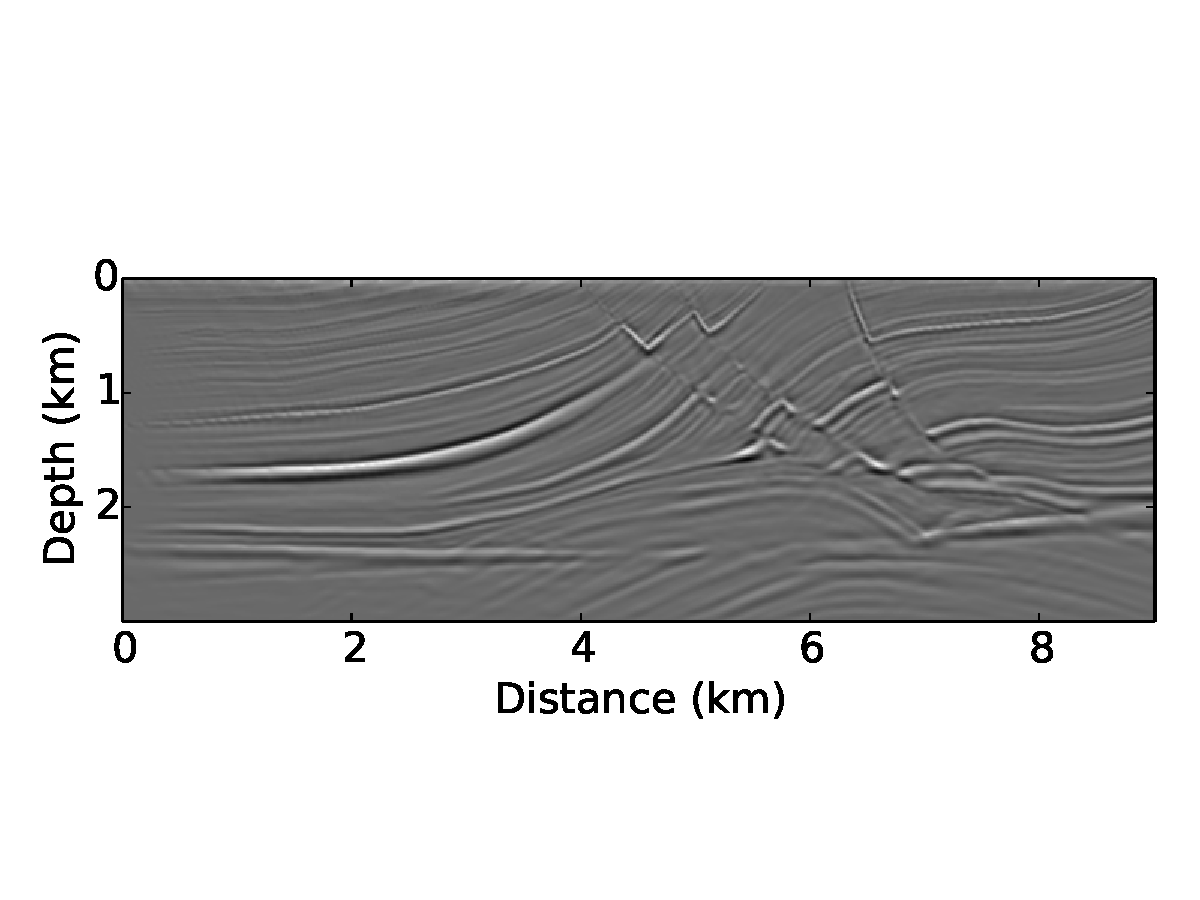
\epsfig{file=Fig/case-5-stack,width=10cm}
\end{figure}
\end{frame}
%------------------------------------------------------
\begin{frame}{Numerical example}
%------------------------------------------------------
Conventional imaging condition:
\begin{figure}
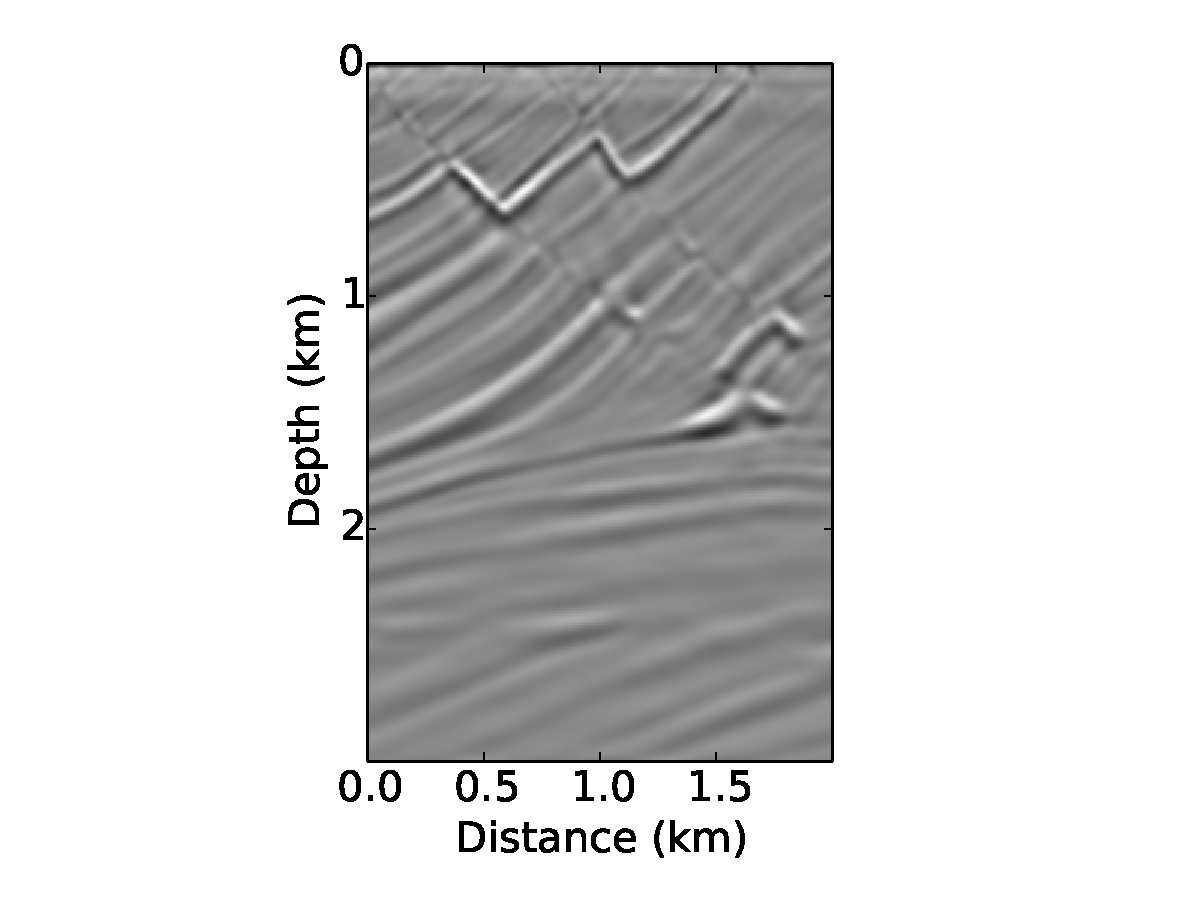
\epsfig{file=Fig/case-4-stack-zoom,width=9cm}
\end{figure}
\end{frame}
%------------------------------------------------------
\begin{frame}{Numerical example}
%------------------------------------------------------
New imaging condition:
\begin{figure}
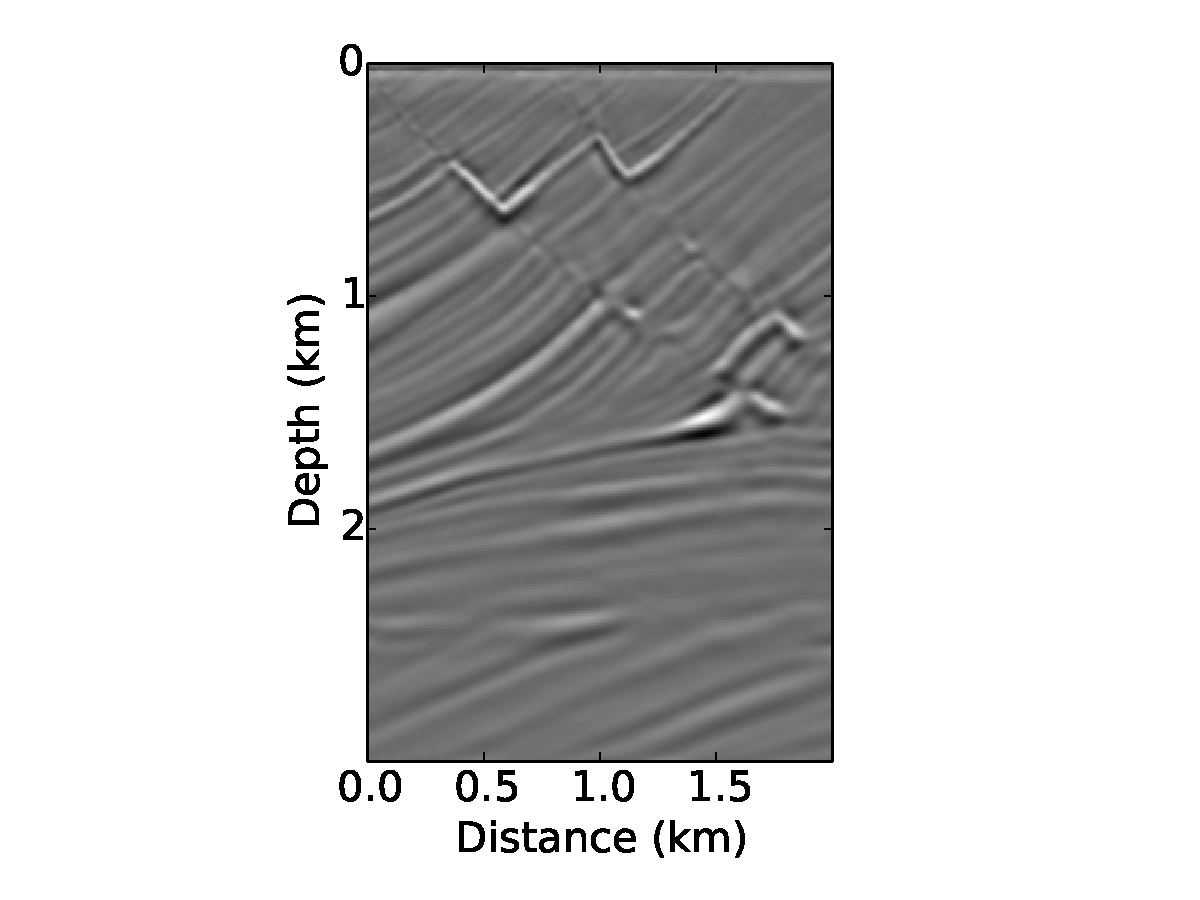
\epsfig{file=Fig/case-5-stack-zoom,width=9cm}
\end{figure}
\end{frame}
\end{document}
